\documentclass{report}

\usepackage{amssymb}
\usepackage{amsfonts}
\usepackage{amsmath}
\usepackage{dsfont}
\usepackage{bm}
\usepackage[a4paper, total={6in,8in}]{geometry}
\usepackage{graphicx}
\usepackage{float}
\usepackage{subcaption}
\usepackage{datetime}
\usepackage{natbib}
\usepackage{hyperref}

%\usepackage{amssymb}
%\usepackage{amsfonts}
%\usepackage{amsmath}
%\usepackage{dsfont}
%\usepackage{bm}
%\usepackage[a4paper, total={6in,8in}]{geometry}
%\usepackage{graphicx}
%\usepackage{float}
%\usepackage{subcaption}
%\usepackage{natbib}
%\usepackage{hyperref}

\graphicspath{{/figures/}{Matlab Demos/sounds/}{voiced_sounds/case_1}{voiced_sounds/case_2}{voiced_sounds/case_3}}

\title{Models for Phonation}
\author{Will Woolfenden}

\begin{document}

\begin{titlepage}
    \begin{center}
        \vspace*{1cm}
            
        \Huge
        \textbf{Models for Phonation}
            
        \vspace{0.5cm}
        \LARGE
        Mathematical Models for Voice Production in Nonlinear Dynamics
            
        \vspace{1.5cm}
            
        \textbf{Will Woolfenden}
        
        \vspace{0.5cm}
        
        $10628968$
            
        \vfill

        Project supervisor: Prof. Oliver Jensen \\

        \vspace{0.8cm}
            %final submission
        Submission for MATH30000 Double Project for the $2022/23$ academic year
            
        \vspace{0.8cm}
            
        \Large

        School of Mathematics\\
        The University of Manchester\\
        United Kingdom\\
        \today
    \end{center}
\end{titlepage}

\begin{abstract}
    A single mass model for phonation considers steady Bernoulli flow through a channel and a vocal fold modelled by a stiff mass.
    The model formulates a second order non-linear ordinary differential equation for the motion of the mass with two parameters.
    Conditions for oscillations can be expressed in terms of the parameters involved,
    and we deduce explicit results involving the stationary equilibrium solutions.
    We formulate the equation as a first order vector ODE and derive the Jacobian matrix for equilibria,
    allowing us to compute eigenvalues which inform us on the stability of these stationary points.
    A two mass model considers the same problem with two stiffness-coupled masses and a quasisteady flow.
    We obtain a fourth order system with four parameters.
    Under strong stiffness coupling, the two masses move as one and are able to replicate the oscillatory behaviour of the single mass model.
    We explore parameter configurations that yield different equilibrium solutions,
    and again construct the Jacobian matrix to analyse the stability of these equilibrium solutions.
    In some cases, we can obtain results analytically.
    We introduce methods to verify solutions through analytical and numerical methods,
    and provide a Fourier analysis of particular results which yield frequency spectra of quasiperiodic motions.
    We end by analysing the results of the two mass model in relation to real phonation and considering how the models could be improved.
\end{abstract}

\chapter{Introduction}
\label{cha:intro}

\section{The concept and process of phonation}

Phonation is a complex human mechanical process in which the vocal cords, being small regions of flexible tissue located in the larynx,
begin to vibrate as air is expelled from the lungs and lower airway passages towards the throat and out of the mouth.
As such, phonation can be regarded as the interation of two processes in the body,
being the exhalation of air from the lungs,
and the forcing of muscles in the larynx.
The extremely rich and varied tones that may be produced form the basis for the production of elongated vowel sounds.

The phonation process begins when air is expelled from the lungs.
The diaphragm contracts, applying a pressure to the lungs which causes air to be driven out.
Air travels through the airways, which have an extremely complicated, inverted tree-like structure,
collecting in the bronchi (single airway per lung) and then trachea (single airway).
Now in the upper airways, the air travels upwards from the trachea, through the larynx, and out of the body through either the nose or mouth.
It is in the larynx that the mechanical process of phonation occurs.
The glottis is the opening in the larynx between the vocal folds,
hence the glottis must be open in order for phonation to occur.
When air travels through the glottis,
a decrease in pressure may cause the vocal folds to oscillate.
When these oscillations occur,
the propagation of the vibrations lead to the production of voiced sounds.

When the glottis closes, it may be that the vocal folds come to rest,
or it could be that the glottis collapses quickly, for example in a pattern of coughing or choking.
In this case, it is important to consider how the vocal folds might collapse but then rebound open again,
and how this would occur.
The vocal folds do not deform in a linearly elastic manner \cite{alipour_2012},
meaning that the rate at which they strain is not directly proportional to the stress they are subjected to.
We could imagine that on a sudden closure of the glottis,
a forcing pressure from the lower airway drives the vocal folds apart again.
Deformations of the vocal folds on collision are one of the features considered in ``Synthesis of voiced sounds from a two-mass model of the vocal cords'' \cite{ishizaka_flanagan_1972},
which will be discussed more in the section on reviewing mathematical models.

The tones produced by the oscillations of the vocal folds produce a harmonic series,
which is the nature of all pitched sounds, such as those produced by musical instruments.
A harmonic series, in this context,
means that the waveform produced by the oscillations is a series on integer-frequency-valued periodic functions,
relative to a \textit{fundamental frequency}.
Conventionally, the mathematical definition of the harmonic series is the infinite sum:
\begin{equation*}
    \hat{W} = \sum_{n=1}^{\infty}\frac{1}{n} = 1 + \frac{1}{2} + \frac{1}{3} + \mathellipsis.
\end{equation*}
The overtone series is the application of the harmonic series to the frequency of oscillations.
If we have a fundamental frequency $\omega$, then we can take a series of periodic functions, in this case sine,
on integer multiples of the fundamental frequency.
We can write this in series form as follows:
\begin{equation*}
    W(x,t) = \sum_{n=1}^{\infty}a_n \sin(ct) \sin(n \omega x).
\end{equation*}
For clarity, $W$ is a function on length $x$ and time $t$.
The wave speed $c$ is the speed at which the waves oscillate in time,
and $\omega$ is their fundamental frequency.
All frequencies $n\omega$ are integer multiples of $\omega$.
We may consider $x$ to be bounded on an interval, such as $[0, \pi]$.
In this case, we can visualise $W$ as a series of waves on a string.
The constant coefficients $a_n$ define the weighting of the linear combination of the periodic functions.
A different bias on different regions of the harmonic series lead to different textures of sound.

When formulating mathematical models,
we will make several assumptions that reduce the complexity of the model,
which make the process of constructing purely mathematical expressions much easier than they would be otherwise.
However, these approximations and assumptions also reduce the complexity of the mathematics we derive,
meaning we lose features that would arise from a model that accommodates more complex features of phonation.
There are two reasons we make these assumptions.
First of all, due to the scope of this project,
certain features must be neglected in order to finalise mathematical relationships that we can analyse in detail.
Furthermore, we want to prioritise certain aspects that we would expect to see from the model,
which in this case is the oscillatory motion of the vocal cords,
and hence it is reasonable to neglect features that are not directly important for this process.
For example, we could neglect terms in equations if their primary importance was describing how the tension on a vocal cord affects the texture of the tone it produces,
since we are not interested in terms which give extremely precise modifications to the oscillations.

\section{Motivation}

Models for phonation provide insight on the mechanics that contribute to real voice production.
Humans do not have conscious control over the vocal folds,
rather the muscles in the larynx work together with the exhalatory pressure from the lungs in order to induce glottal oscillations.
As such, producing a model for phonation means we can begin to understand the mechanics of the process.

Our goal is to formulate a model for phonation,
which we wish to can analyse to obtain mathematical descriptions of real voice production.
This can be divided into several sections.
First, we will briefly discuss the principles of mathematical modelling in fluid mechanics,
so we have a strong foundation before building our models.
When we are constructing a mathematical model,
we will be able to understand how different assumptions in the basic fluid mechanics lead to different components of the model.
Finally, this carries through into the analysis of the model,
allowing us to make links between the results a model provides,
and the mechanical properties that cause these behaviours.
If we produce a model starting with only fundamental mechanics,
then we can more easily understand which components of the model merit which features that arise in our analysis.
This means we have clear links between the physics that forms our model,
and the properties of our results.

Once we have a model,
there are many directions that can be explored to develop our study,
A mechanical model can act as a foundation for synthesis of speech \cite{ishizaka_flanagan_1972},
where we would apply mathematical principles of sound wave propagation.
Phonation is affected by plenty of factors outside of the glottal region itself,
most notably the resonance coming from the structure of the lower and upper airways as well as the mouth.
The models we explore are simplified,
and more generally study the properties of Bernoulli flow in wind tunnels.
These have applications to the study of fluid mechanics and aerodynamics of channel flows.

\section{Modelling phonation}

As discussed, we will make limitations to the mathematical models we consider,
to refine the model into something we can feasibly analyse while also gaining interesting results.
First of all, while inspiratory phonation (inspiration) differs from expiratory phonation (exhalation),
we will only focus on the expiratory flow case.
In the construction of the model, the cases turn out to be identical up to symmetry anyway.
We will also simplify the geometry of a model of the larynx,
reducing the problem to the flow through a cuboid, with a vocal fold modelled by a movable wall on the side of the channel.
The motion of the wall can be restricted by Hooke springs, and we can control their properties.

We will also assume either a steady or quasisteady flow.
While it is entirely possible for the flow in real speech to be turbulent and not steady,
assuming otherwise allows us to apply Bernoulli's equation for a steady flow,
which gives a simple yet powerful statement on the relationship between pressure $p$, density $\rho$ and flow velocity $\mathbf{u}$.
Restricting our investigation to incompressible fluids, namely where $\rho$ is constant,
provides similar simplifications to our analysis.

Due to the symmetry of the vocal tract,
we can simplify our analysis by only studying one side,
since accommodating both sides in our model would only provide insight under asymmetric forcing terms or initial conditions.

Further assumptions we consider are the one-dimensional motion of the modelled vocal folds,
the elasticity being linear and modelled by Hooke springs,
and a simple geometry for the vocal tract. 

\section{Literature review for mathematical models of phonation}

The paper ``Synthesis of voiced sounds from a two-mass model of the vocal cords'' \cite[1972]{ishizaka_flanagan_1972} is arguably the most important work of research in the field of mathematical models for phonation.
In their research, Ishizaka and Flanagan devise a two-mass model for the vocal cords, and then compute results to generate synthesised voiced sounds.
The model consists of two masses to represent a vocal fold, which are stiffness coupled, comprising the wall of a channel.
A flow passes through the channel and sound waves propagate from the planes,
and the approximation to voiced sounds is computed as the result of the waves transmitted. %% bit more on wave physics maybe

The two mass model is an extremely simple yet insightful model,
which generates behaviours of seemingly erratic oscillations.
The main body of this project is the formulation and analysis of a two mass model.

In the mathematical study of phonation, the myoelastic and aerodynamic theories suggest the nature of the production of voiced sounds.
The myoelastic theory assumes that the vocal cords repeatedly close,
each time being driven apart by the pressure from the forced airflow from the lower airways,
and the frequency of this repeated process determines the frequency of the voiced sounds.
The aerodynamic theory instead applies the properties of pressure in a fluid flow,
imposing that a pressure drop in the glottis leads to sustained oscillations of the vocal cords.
This kind of pressure drop is often referred to as \textit{Bernoulli pressure}, which will be discussed in more depth later.
It is commonly believed that both theories are involved in the production of voiced sounds,
and the ideas are discussed by Titze in ``Comments on the myoelastic-aerodynamic theory of phonation'' \cite[1980]{titze_1980}.
Titze is an extremely prominent author in the field of voice and hearing in mathematical modelling.

The research paper ``Theory and measurement of snores'' \cite[1993]{gavriely_jensen_1993} involves a model which is not designed to approximate phonation.
Rather, its purpose is to provide mechanical insights to the factors present in obstructive sleep apnea.
However, the model itself can be applied to the investigation of phonation,
being a single mass in the wall of a channel subject to stiffness and Bernoulli pressure.
One of the authors, Oliver Jensen, is the supervisor for this project.

Mathematical models for the vocal folds are often heavily simplified, and hence some features of natural phonation are lost.
In ``Synthesis of breathy, normal, and pressed phonation using a two-mass model with a triangular glottis'' \cite[2011]{birkholz_2011},
the authors construct a model for phonation which considers a glottis of a particular shape, which is able to close gradually.
The model is able to synthesise more modes of voiced sounds than traditional models,
particularly being able to produce the range of sounds from ``breathy'' speech (soft-spoken, close to whispering) to ``pressed'' (tense, thin). 

\section{Principles of fluid mechanics}

Euleriean fluid mechanics in a Cartesian coordinate system defines a flow $\mathbf{u}=(u_x,u_y,u_z)$ in a $2$D or $3$D domain,
which is a function of position $\mathbf{r} = (x,y,z)$ and time $t$.
We will describe the $3$D case.
As well as a flow $\mathbf{u}$,
we have fluid density $\rho$ and pressure $p$,
which are often functions of position and time.
In the cases we will study,
we assume the flow is imcompressible,
meaning $\rho$ is uniform across the domain of the flow.
This may appear like a restrictive assumption,
but we still obtain rich and interesting mathematical results from the analysis of an incompressible flow.

The Eulerian framework fundamentally describes the flow field, not the fluid it contains.
The change in a property $\bullet$ of a fluid object must be found using the material derivative
\begin{equation}
    \frac{D\bullet}{Dt} = \frac{\partial \bullet}{\partial t} + (\mathbf{u}\cdot \nabla)\bullet
\end{equation}
where $\nabla$ is the vector differential operator.

A steady flow is a flow $u$ which is independent of time.
The streamlines in a steady flow are fixed, and are identical to the paths taken by a supposed particle placed into a flow at any time.
Bernoulli's equation for a steady flow is as follows:
\begin{equation}
    \frac{1}{2}|\mathbf{u}|^2 + \Omega + \int\frac{\mathrm{d}p}{\rho} = \mathrm{constant~along~a~streamline}.
\end{equation}
The term $\Omega$ is the potential for the body forces on the fluid, such as gravity.
If the potential is either zero or constant,
then $\Omega$ cancels when applying Bernoulli's equation since the body forces $\mathbf{F} = \nabla \Omega$ are zero. %plurals
For our research, we will assume there are no body forces and thus neglect $\Omega$.
Bernoulli's equation is extremely useful, since it gives us a relationship between fluid velocity and pressure in a steady flow.

Fluid mass flux $Q$ at a given cross-section is the rate at which fluid mass passes through the region,
given in terms of an integral:
\begin{equation*}
    Q = -\iint_A \rho \mathbf{u} \cdot \mathbf{n} \mathrm{d}S,
\end{equation*}
where $\mathbf{n}$ is the outer unit normal to a cross-section.
By convention, the outer unit normal points away from the volume,
hence in the opposite direction of the flow, thus we require the negative sign.
This leads to the principle of conservation of mass, where the net flux entering a volume $V$ is the same as the rate of change of fluid mass within that volume.
The net flux is the flux out minus the flow in.
This can be formally expressed as follows
\begin{equation*}
    \iiint_V \frac{\partial\rho}{\partial t} \mathrm{d}V = - \iint_A \rho \mathbf{u} \cdot \mathbf{n} \mathrm{d}S 
\end{equation*}
We can combine conservation of mass with the fact that for an incompressible fluid,
the material derivative of density $D\rho / Dt$ is zero.
We obtain an expression for incompressibility
\begin{equation*}
	\nabla \cdot \mathbf{u} = 0.
\end{equation*}

In this research project, the models we will consider involve simplified geometry and more straightforward assumptions of mechanics in comparison to some of the literature we have acknowledged.
Fundamentally, we want to consider a fluid flow through a rigid channel, and suppose that a region of wall has freedom of motion in one dimension normal to the flow.
It is appropriate to introduce the definition of a \textit{plug flow}, being a fluid flow through a channel in which the flow is uniform over cross-sections through the channel.
The plug flow model is a general form for the simple geometry channel flow models we will consider throughout this project.
We will only discuss a case for a two-dimensional flow, since the intricacies are not vital to our analysis.
Assume an incompressible steady flow \(\mathbf{u}(x)\) travels through a channel in the positive $x$ direction and has zero velocity in the $y$ direction.
such that the horizontal $x$ length $L$ of the flow is much larger than vertical $y$ width $W$.
We assume the flow is uniform over a cross section.
We can evaluate flux over a cross-section with length/area $A$
since velocity is uniform over said cross section, and we obtain
\begin{equation}
	Q(x) = -\int_W \rho \mathbf{u}\cdot \mathbf{n} dS = WU
\end{equation}
where $U = \mathbf{u}(x) \cdot \mathbf{e}_x $ at the point in the path of the flow normal to the cross section.
The elementary vector $\mathbf{e}_x$ is the unit vector in the positive $x$ direction.
Velocity still may change in $x$, for example if the flow is driven by a pressure gradient in the $x$ direction.
This gives us a very flexible method to express the fluid flux in a rigid channel.

\section{Principles of non-linear dynamics and dynamical systems}

The modelling of phonation uses techniques from analysing systems of differential equations.
The study of dynamical systems, as far as we are concerned,
involves studying systems of differential equations that describe time-dependence in a model,
and provides insight into characteristics of a model such as equilibrium solutions and classes of behaviours.
In Chapter \ref{cha:onemass}, we study a single mass model to approximate a vocal cord,
and in Chapter \ref{cha:twomass} we generalise into a two mass model and obtain a fourth order system of differential equations.
In all cases the equations of motion are autonomous and non-linear.
Consider the example on two variables \((x,~y)\), being
\begin{equation}
    \begin{aligned}
        \frac{\mathrm{d}x}{\mathrm{d}t} &= f(x,y) \\
        \frac{\mathrm{d}y}{\mathrm{d}t} &= g(x,y).
    \end{aligned}
\end{equation}
In this example,
the equations are autonomous,
which will be the case for all problems considered in this report.
The \textit{phase portrait} is the representation in which the coordinate axes are the variables $x,y$,
which can be generalised to higher dimensional cases,
but cannot be fully visualised for dimensions higher than three.
We use phase-portrait representation as an alternative visualisation of the behaviour of a system.
If a variable $x$ is governed by an ODE,
we plot its behaviour over time where the different axes represent velocity $dx/dt$ against position $x$,
rather than just visualising position against time.
The phase-portrait is a useful method of representation for problems in dynamical systems,
since an ODE or system of ODEs can be characterised by the locations and properties of its stationary equilibria.
This alternative approach allows us to construct visualisations that show some characteristics of a system more clearly, such as the radii of different closed orbits,
and the positions of equilibrium solutions.
The path we visualise in the phase portrait is a curve of the behaviour of the system parameterised by time $t$. 
Representation of solutions in the phase portrait will be vital to our analysis of our models.

If the equations \(f\) and \(g\) are non-linear,
we can't do much to solve this equation.
Aside from producing numerical computations, we could look intuitively for equilibrium solutions \((x,y) = (x_0,y_0)\),
which are fixed point solutions for which all time derivatives of \(x\) and \(y\) are zero.
Hence equilibrium solutions are equivalently solutions to the homogeneous couple \(f(x,y) = 0,~g(x,y) = 0\).
Close to an equilibrium solution,
we would expect the functions' behaviour to be well approximated by their first order Taylor Series approximations, being
\begin{equation}
    \begin{aligned}
        f(x,y) &\approx f(x_0,y_0) + (x-x_0)\frac{\partial f}{\partial x}(x_0,y_0) + (y-y_0)\frac{\partial f}{\partial y}(x_0,y_0) \\
        g(x,y) &\approx g(x_0,y_0) + (x-x_0)\frac{\partial g}{\partial x}(x_0,y_0) + (y-y_0)\frac{\partial g}{\partial y}(x_0,y_0).
    \end{aligned}
\end{equation}
The constant terms disappear since \(f, g\) are zero at an equilibrium by definition.
As $(x,y) \rightarrow (x_0,y_0)$, the terms of order $n > 1$ approach zero,
and the most significant terms are those involving the first partial derivatives.
We obtain the approximation for the system local to an equilibrium solution,
\begin{equation}
    \begin{aligned}
        \frac{\mathrm{d}x}{\mathrm{d}t} &= \left(\frac{\partial f}{\partial x}(x_0,y_0)\right)(x-x_0) + \left(\frac{\partial f}{\partial y}(x_0,y_0)\right)(y-y_0) \\
        \frac{\mathrm{d}y}{\mathrm{d}t} &= \left(\frac{\partial g}{\partial x}(x_0,y_0)\right)(x-x_0) + \left(\frac{\partial g}{\partial y}(x_0,y_0)\right)(y-y_0),
    \end{aligned}
\end{equation}
which is a system of linear equations.
For convenience, we make the substitutions \(u = x-x_0,~v = y-y_0\) which are linear substitutions proportional to the variables of interest \((x,y)\).
Hence the above approximation is equivalent to the following matrix equation:
\begin{equation}
    \frac{\mathrm{d}}{\mathrm{d}t} \begin{pmatrix}
        u \\
        v
    \end{pmatrix} = \begin{bmatrix}
        \frac{\partial f}{\partial x}(x_0,y_0) & \frac{\partial f}{\partial y}(x_0,y_0) \\
        \frac{\partial g}{\partial x}(x_0,y_0) & \frac{\partial g}{\partial y}(x_0,y_0)
    \end{bmatrix} \begin{pmatrix}
        u \\
        v
    \end{pmatrix}.
\end{equation}
Letting \(\mathbf{u} = (u,v)^\mathrm{T}\) and writing \(J\) as the matrix of derivatives,
we can write the matrix equation compactly as \( \dot{\mathbf{u}} = \mathbf{Ju}\), where the dot denotes the time derivative.
The matrix \(\mathbf{J}\) is the \textit{Jacobian matrix}.
The Hartman-Grobman Theorem in dynamical systems tells us a very important result,
being that the behaviour of the system near the stationary point can be determined by computing the Jacobian matrix \(\mathbf{J}\) at the equilibrium solution,
and computing the eigenvalues of the matrix.
The Jacobian is often a sparse matrix, and its eigenvalues are often complex.
For every equilibrium solution, we must compute the Jacobian and its eigenvalues in order to determine the behaviour of the system at all equilibrium points.
For clarity, the eigenvalues of the Jacobian are the constant terms \(\lambda\) that solve the equation \( \mathbf{J} -  \lambda \mathbf{I} = \mathbf{0}\),
where \(\mathbf{I}\) is the appropriate size identity matrix.
This also concerns the problem of finding equilibrium solutions in the first place, which is usually non-trivial.
Importantly, the vector $\mathbf{u}$ is defined on the independent variables $u,v$ which map one-to-one to the vectors which define the phase portrait.
Hence, eigenvectors of the matrix $\mathbf{J}$ are vectors in the phase portrait from equilibrium solutions,
hence they affect behaviours of the system near these stationary points.

The most important result on eigenvalues of equilibria is that an equilibrium solution is unstable if any of its eigenvalues have positive real part.
Recall that the linearisation of the system is of the form
\begin{equation}
	\dot{\mathbf{u}} = \mathbf{Ju}.
\end{equation}
If $\mathbf{J}$ has an eigenvalue $\lambda$ for an eigenvector $\mathbf{u}_0$,
then we can model the trajectory from this eigenvector by the ODE and initial condition
\begin{equation*}
	\begin{aligned}
		\dot{\mathbf{u}} &= \lambda \mathbf{u}, \\
		\mathbf{u}(t=0) &= \mathbf{u}_0.
	\end{aligned}
\end{equation*}
This is a first order vector ODE and has a general solution
\begin{equation}
	\mathbf{u} = \mathbf{u}_0 e^{\lambda t}
\end{equation}
and hence the value of $\lambda$ determines the trajectory from the initial point $\mathbf{u}_0$.
If $\lambda$ has a positive real part then the trajectory diverges exponentially from the equilibrium and hence the equilibrium is unstable.

For a more rigorous understanding of the linearisation of a system of equations and an understanding of the Hartman-Grobman Theorem,
see \cite{perko_textbook_1996},
particularly sections 1.1 on simple examples of linear systems,
1.5 on two-dimensional linear systems,
1.9 on the theory of stability,
and 2.6 on linearisation.

\section{Housekeeping}

We will briefly discuss the notation used and any preliminary notes on methods.
Within a chapter, all notation will be almost completely consistent,
however variables are not consistent across separate chapters.
For example, we use $\mu$ as a parameter for the single mass model,
and denote eigenvalues of the Jacobian with $\lambda$,
however in the two mass model we use $\lambda$ as a parameter and thus it cannot be used to also denote eigenvalues,
so we denote eigenvalues with $\sigma$ instead.

The only significant inconsistency in our writing is when we derive the two mass model.
We denote the dimensional dependent variables $h_1,h_2,$
and analyse the model to obtain the dimensionless variables $\hat{h}_1,\hat{h}_2.$
Once we have obtained the ODEs in nondimensional form,
we won't consider the dimensional variables again,
so for simplicity we change back to writing the independent variables as $h_1,h_2$,
but use them to denote the nondimensional quantities.
We do the same for all the nondimensionalised variables in the problem.

The computations in this project are all performed in MATLAB,
using the $64$-bit double precision floating point arithmetic standard.

\section{Structure}

The first section of this project studies the single mass model from ``Theory and measurement of snores'' \cite{gavriely_jensen_1993},
which is a model formulated to consider the factors involved in obstructive sleep apnea.
We will find that the features derived in the model are very relevant to the investigation of phonation,
and that this single mass model serves as a strong basis for more generalised models.

In the second section, we generalise the single mass model into a structure in which two masses model a single vocal cord,
where the masses have a component of stiffness coupling between them.
This model builds on the single mass model,
but also takes strong inspiration from the two mass model formulated in ``Synthesis of voiced sounds from a two-mass model of the vocal cords'' \cite{ishizaka_flanagan_1972},
which discusses the formulation of a mathematical model for the purpose of generating artificial speech using a computer.
The formulation and study of the two mass model is the largest and most important part of work contained in this project.
After having investigated the single mass model and the two mass model,
we will review the approximations and simplifications made during the formulation processes and suggest refinements to the models.
We conclude by discussing the results, which are the insights to the nature of phonation that we have gained from inspecting the behaviours of the models.

\documentclass{article}

\usepackage{amssymb}
\usepackage{amsfonts}
\usepackage{amsmath}
\usepackage{dsfont}
\usepackage[a4paper, total={6in,8in}]{geometry}
\usepackage{graphicx}
\usepackage{float}
\usepackage{hyperref}

\graphicspath{{figures/}}

\title{MATH30000 Project - Phonation}
\author{Will Woolfenden}

\begin{document}

\maketitle

\section{Introduction}

\subsection{Definitions}

Phonation is the human process in which respiratory exhalation and vocal cord oscillations work together to produce sounds that we identify as spoken words.
Air is projected from the lungs in a fluid motion through the airways.
When passing through the larynx, the forced oscillations of the contained vocal cords interact with the air particles and induce the sound of speech.

The goal of this project is to explore models of the phonation process.



\section{Principles of the single-mass model}

\subsection{Derivation}

% TODO: Add figure of the model schematic

The first model we will study is taken from Theory and Measurement of Snores \cite{gavriely_jensen_1993}.
It models the inspiratory process, designed to investigate snoring as a symptom of obstructive sleep apnea.
The model proposes that the inspiratory path consists of first a region of the upper airway,
which has a given viscous resistance.
Then, there is a region of a channel between two walls of given area, where one wall is a suspended plate rather than being fixed in place.
The term we wish to investigate is $b$, which describes the positive displacement between the fixed wall and the suspended wall opposite.
The walls themselves are assumed to be of equal dimensions, and behave such that the surfaces are always parallel to each other.
Also necessary to note is that the plate may only move in the direction of $b$ which is the normal to its surface,
hence $b$ measures the only degree of freedom of the plate's motion.

%figure on diagram of the model

The oscillations in $b$ that may take place, depending on conditions, is the subject of our analysis.
In the original paper, the oscillations are regarded as snores,
whereas here they will be regarded as the production of phones.
The idea is the same, since the mathematical principles applied in the definition of the model are not exclusive in any way to particular studies of sleep apnea or the like.

Oscillations are the event where, given certain constraints, $b$ will exhibit simple harmonic motion. %maybe cite here
In the model provided, indefinite oscillations can very much be observed given the right conditions,
however it is important to be aware of some properties of the model,
namely the region in which our attention is focussed. Given physical attributes are associated with the model,
and so, for example, behaviours of $b$ when negative are ignored in the investigation.

There are three forces acting on the plate in the airway, which govern the motion we are investigating.
The plate is suspended in place by an elastic force $F_k$, namely a conventional Hooke spring with spring constant $k$.
This spring force suspends the plate such that it resists the closure of the airway,
so the tension force on the plate is acting tangent to the direction of positive displacement of the plate.

% schematic with opposing walls and illustration of spring direction.

Since the upper airway has a resistance $R$ to the inspiratory fluid flow,
this leads to a pressure drop in the airways. %TODO: Explain this

An internal increase in pressure would produce an outward force on the airway,
which in this model would be tangent to the positive displacement direction.
Since there is instead a \textit{decrease} in pressure, an inward force is resultant,
in the direction tangent to the negative displacement. We label this force as $F_p$.
Pressure itself is the force per unit area,
so the value of the force $F_p$ is the pressure multiplied by the surface area of the plate.

The final force to consider in the motion of the plate is consequence of Bernoulli's principle,
namely that along a streamline, in a steady flow,
the sum of the kinetic energy and the potential energies, per unit mass, are constant.
In Bernoulli's equation (Equation \ref{eqn:bernoulli}), $1/2\mathbf{u}\cdot\mathbf{u}$ is the fluid kinetic energy per unit mass,  %some of this is wrong
$\Omega$ is the potential energy per unit mass of the body forces of the fluid,
and $\int dp/\rho$ is the inner potential energy, regarding that $p$ and $\rho$ are either constant or codependent.

\begin{equation}
    \frac{1}{2}\mathbf{u}\cdot\mathbf{u} + \Omega + \int\frac{dp}{\rho} = C
    \label{eqn:bernoulli}
\end{equation}

%this is where the explanation gets dodgy - this could be completely wrong. if so, then the bernoulli effect force is more likely the increase in fluid ke when a constriction leads to an increase in pressure
In order to apply Bernoulli's principle to find the pressure, we simply rearrange the equation for $p$.
We obtain $F_b$ by again multiplying the pressure by the cross-sectional area of the plate.

%include some derivation for $P_b$?

The governing equation of the model is derived from Newton's second law.
Given that the plate has a mass $m$, we know the three forces acting on it,
and so the initial equation of motion can be expressed as

\begin{equation}
    m\frac{d^2 x}{dt^2} = F_e - F_p - F_b.
    \label{eqn:model_init}
\end{equation}

This is not the principal equation of the model,
since the terms should be nondimensionalised and normalised.
For example, $x$ measures displacement,
but it is not stated under what scale.
Furthermore, the terms for the forces are all products of pressure and their dimensional properties,
meaning they measure in units that would ideally be reduced.
We can normalise $x$ by defining $b = x/x_0$, where $x_0$ is the resting position of the plate under particular circumstances. %TODO: amend this!! what are the particular circumstances??
The forces can be nondimensionalised by dividing by the areas or volumes they are acting over.
Resultingly, we produce the governing equation for the positive displacement of the channel wall from collapse at $0$,

\begin{equation}
    \frac{d^2b}{dt^2} = 1 - q - b - \frac{\mu q^2}{2b^2}
    \label{eqn:master}
\end{equation}

where $\mu, q$ are parameters linked to the forces acting on the channel wall.

%plan is to have this chapter just discuss individual properties of the model with analysis where relevant. Will include matrix method. Then in next chapter we introduce KE graphs in the phase-plane.

\subsection{Nonlinearity}

It is important to note the properties of Equation \ref{eqn:master} before developing analysis.
The equation itself is a second order, nonlinear, autonomous, inhomogeneous ODE.
The property of nonlinearity is due to the existence of the $\mu q^2/2b^2$ term.
Due to the equation being nonlinear, regular methods for solving ODEs are far less powerful,
and the properties of solutions are different to regular linear ODEs.
Most importantly, while linear ordinary differential equations often possess unique solutions subject to boundary or initial conditions,
the same does not apply in the case of nonlinear equations.

We will first demonstrate the implications of nonlinearity by attempting methods suitable for linear ODEs,
in which we do not expect to solve the ODE but instead use for demonstration.
Note the absence of the $db/dt$ term in the governing equation.
We can attempt the method of reduction by proposing a substitution $v=db/dt$ and forming a first order ODE.
First, note that

\begin{equation}
    \frac{dv}{dt} = \frac{dv(b(t))}{dt} = \frac{dv}{db}\frac{db}{dt} = \frac{dv}{db}v,
\end{equation}

and hence (while assuming commutativity),

\begin{equation}
    v \frac{dv}{db} = 1 - q - b - \frac{1}{2}\mu q^2\left( \frac{1}{b^2} \right).
\end{equation}

Assuming we can separate the variables, we can write an indefinite integral equation and obtain an expression for $v$, namely

\begin{equation}
    \begin{aligned}
        \int v~dv = \int \left(1 - q - b - \frac{1}{2}\mu q^2 b^{-2} \right) db \\  %TODO: edits. separate all this mess.
        v^2 = \left(\frac{db}{dt}\right)^2 & = 2b(1-q) - {b^2} + \mu q^2 b^{-1} + C_1, %we have integrated AND multiplied by 2.
    \end{aligned}
    \label{eqn:first_order_reduction}
\end{equation}

obtaining a constant of integration $C_1$.
We now have a first order differential equation on $b$, %however we can't solve it because no
but this equation is even harder to reduce or even solve, as we only have the form $v^2 = g(b)$,
where the first derivative is expressed explicitly but not linearly.
Therefore, statements of existence and uniqueness for solutions of ODEs,
which we are accustomed to,
do not hold in the situation where the differential equation is non-linear.

We could have deduced this from the explicit form of Equation \ref{eqn:master},
but this section serves for illustration to aid the reader's understanding of why we cannot analytically solve this ODE.
Additionally, the equation of the form $v^2 = g(b)$ will be useful later.

\subsection{Autonomy}

\begin{figure}
    \centering
    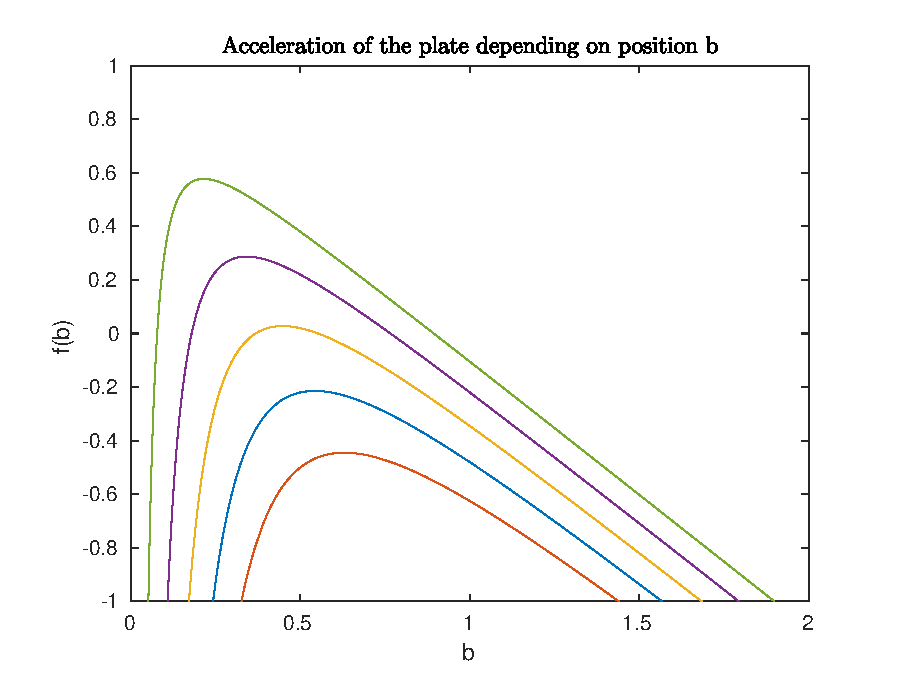
\includegraphics[width=0.5\linewidth]{f_plot_mu_1_q_vary}
    \caption{A plot of the function $f(b) = 1-q-b-\mu q^2/2b^2$ where $\mu=1$, $q$ ranging from $0.1$ (orange) to $0.5$ (green).}
    \label{fig:acc_b_plot}
\end{figure}

The reader may notice that the Equation \ref{eqn:master} is an autonomous ODE,
namely that the independent variable $t$ itself does not appear.
If we let $f$ be a function of $b$ equal to the right-hand side of the equation,
we can produce a plot of the behaviour of $f(b)$ against $b$,
and since the equation is autonomous, this behaviour is not affected by position in time.
Figure \ref{fig:acc_b_plot} shows a plot of $f(b)= 1 - q - b - \mu q^2/2b^2$ against $b$.

This plot allows us to deduce some intuition about the behaviour of $b$.
At a point $b=b_0$, the function $f(b_0)$ is equal to the outward acceleration of the plate.
We can see that $f$ tends towards negative infinity both as $b\rightarrow 0$ and as $b\rightarrow\infty$,
and that for certain $\mu, q,$ there is a positive region of $f$.
Hence if $b$ is either small or large, it will accelerate to closure,
whereas for a range of intermediate values it may accelerate outwards instead.
It is possible under certain conditions for $b$ to behave similarly to a harmonic oscillator,
where its position and acceleration move back and forth reciprocally.

Note that the plot of $f(b)$ does not account for velocity.
Different initial conditions could cause $b$ to behave differently under the same acceleration.

We will start by analysing the properties of the $f(b)$ curve.
In order for there to exist a region of $f(b)$ that takes positive values,
the local maximum of $f(b)$ must be greater than zero.

\begin{align}
    f(b)              & = 1 - q - b - \frac{\mu q^2}{2b^2} \\
    \Rightarrow f'(b) & = -1 + \frac{\mu q^2}{b^3},
\end{align}

from which we can deduce that the maximum is located at the point where $b^3 = \mu q^2$.
If we plug this back into $f$, we can deduce the condition

\begin{align}
    f((\mu q^2)^{\frac{1}{3}}) & = 1 - q - (\mu q^2)^{\frac{1}{3}} - \frac{\mu q^2}{2(\mu q^2)^{\frac{2}{3}}} \\
                               & = 1 - q - \frac{3}{2}(\mu q^2)^{\frac{1}{3}}.
\end{align}

We obtain the result

\begin{equation}
    1 - q - \frac{3}{2}(\mu q^2)^{\frac{1}{3}} > 0.
    \label{eqn:osc_condition}
\end{equation}

If Equation \ref{eqn:osc_condition} is satisfied,
then there exists a region of $f$ which is positive.
Hence if this condition is met then oscillations may occur. %% I feel this should be more rigorous - we haven't proved that this is the condition for oscillations to occur.
We have not yet provided the results to justify this statement, but in the next section we will provide rigorous arguments. % this is my backup argument for now.
Further on, we will be regularly making the assumption that this condition is satisfied,
and hence that oscillations can occur,
in order to develop our analysis of the model.

% Clearly $f$ represents acceleration of the movable wall as a function of displacement $b$. We are only ever concerned with positive $b$ due to the assumptions of the model.
% $f'$ is monotone decreasing, so there may be an interval $I_0=(p,q)$ such that if $b\in I_0$
% then $f$ is positive i.e. $p,q$ are the zeroes of $f$.
% It is not certain that $f$ will have a positive region,
% and this is decided by the parameters $\mu$ and $q$.
% Particularly, we require that the maximum of $f$ ($f'(b_c) = 0$) is greater than zero:

If the acceleration of the channel wall is positive, then the wall will accelerate outwards,
however the acceleration will have to oscillate from positive to negative in order for there to be oscillations in the position itself.
Unlike the simple harmonic oscillator $d^2 x/dt^2 + x = 0,$ the values of $b$ we consider are strictly positive.

\section{Analytical methods for the single-mass model}

%introduce the parameter space
%first discuss configuring the system of differential equations in MATLAB
%introduce phase portrait to compare with distance/time
%integral to the kinetic energy curve graph, recalling earlier result
%matrix method with eigenvectors in the phase plane

%after this is the chapter on developing the single mass model.
%damping
%we assumed steady bernoulli flow for an unsteady problem

\subsection{The parameter space}

\begin{figure}
	\centering
	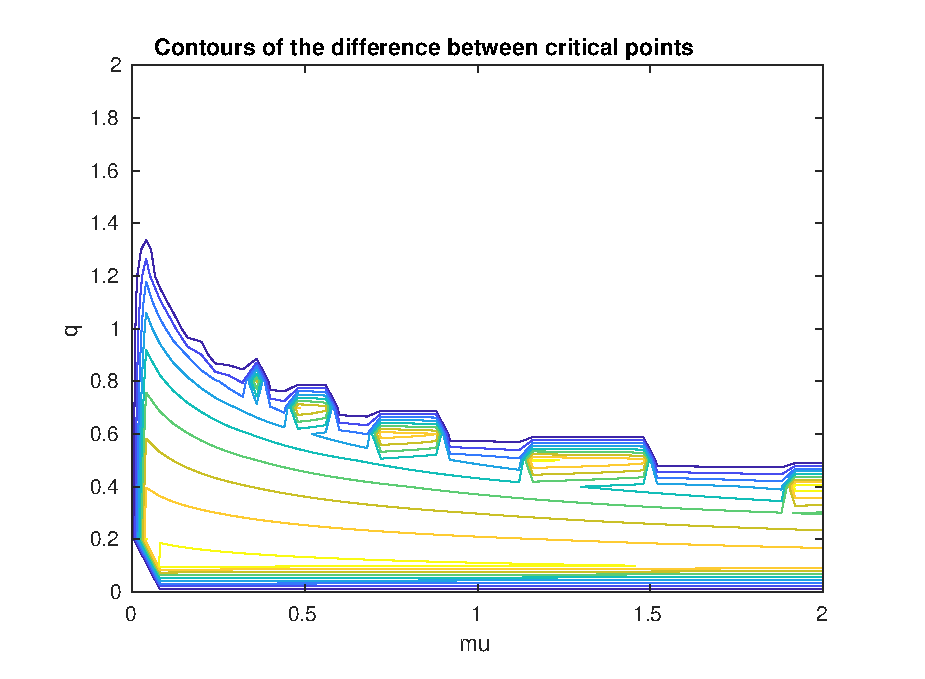
\includegraphics[width=\linewidth]{param_space}
	\caption{A contour graphic of the parameter space. The displacement of $Z$ over a point $(\mu,q)$ represents the distance between critical points for the corresponding form of Equation \ref{eqn:master}.}
	\label{fig:param_space}
\end{figure}

Recall the result obtained in Equation \ref{eqn:osc_condition}.
We can produce a graph (see Figure \ref{fig:param_space}) where $\{\mu, q\}$ is the basis for the plane, and plot the distance between points.
Note that, by the properties of the derivation of the model,
$\mu$ and $q$ must be strictly positive,
hence we are only considering points in the quarter-plane.
Any suitable form of Equation \ref{eqn:master} can be placed in this region,
and if that version exists within a particular contour,
then oscillations may occur in a region of proportional scale.
Around the edges of the curve, the points bifurcate,
which is equivalent to the curve $f(b)$ only having one real-valued zero.

We can gain interesting and useful results regarding sufficient values of $\mu, q$,
most noticeably that for any positive $\mu$, there exists some $q$ such that oscillations may occur.
This relation is not symmetric - $q>1$ immediately breaks the condition.
It is relatively simple to deduce this, since if the $1-q$ term of Equation \ref{eqn:osc_condition} is negative,
the $-3(\mu q^2)^{1/3}/2$ term will always be negative and thus the condition fails.

\subsection{Solving differential equations in MATLAB}

We use MATLAB, primarily the \texttt{ode45()} function, to compute solutions numerically.
However, the governing differential equations must be provided as a first order system.
Equation \ref{eqn:master} can be given in the following form:

\begin{align}
    \frac{db}{dt}       & = \dot{b}                          \\
    \frac{d\dot{b}}{dt} & = 1 - q - b - \frac{\mu q^2}{2b^2}
    \label{eqn:first_order_system}
\end{align}

By using \texttt{ode45}, MATLAB performs numerical integration on all the equations in the system,
thus giving numerical solutions for $b$ and $\dot{b}$ in terms of time $t$, subject to initial conditions.
In most cases, we will consider the plate moving from rest ($\dot{b}(t=0) = 0$) given an initial position $b=b_0$.
Working examples are available in the Appendix.

\subsection{Representations of solutions of differential equations}

The phase-portrait is the vector space spanned by the vectors $b$ and $\dot{b}=db/dt$.
We use phase-portrait representation as an alternative visualisation of the behaviour of motion. If a variable $x$ is governed by an ODE,
we plot its behaviour over time where the different axes represent velocity $dx/dt$ against position $x$,
rather than position against time.

This alternative approach allows us to construct new visualisations of paths taken by the modelled plate.
Paths in phase-plane representation have direct correspondence to plots in position against time.

% phaseplane curves are mu=1, q=0.2 at b=0.1, b_0 ~= 0.1795, 0.3, 0.5
% figures C and D at mu=1, q=1, b = 0.2, 0.4, 0.6, 0.8

\begin{figure}
    \centering
    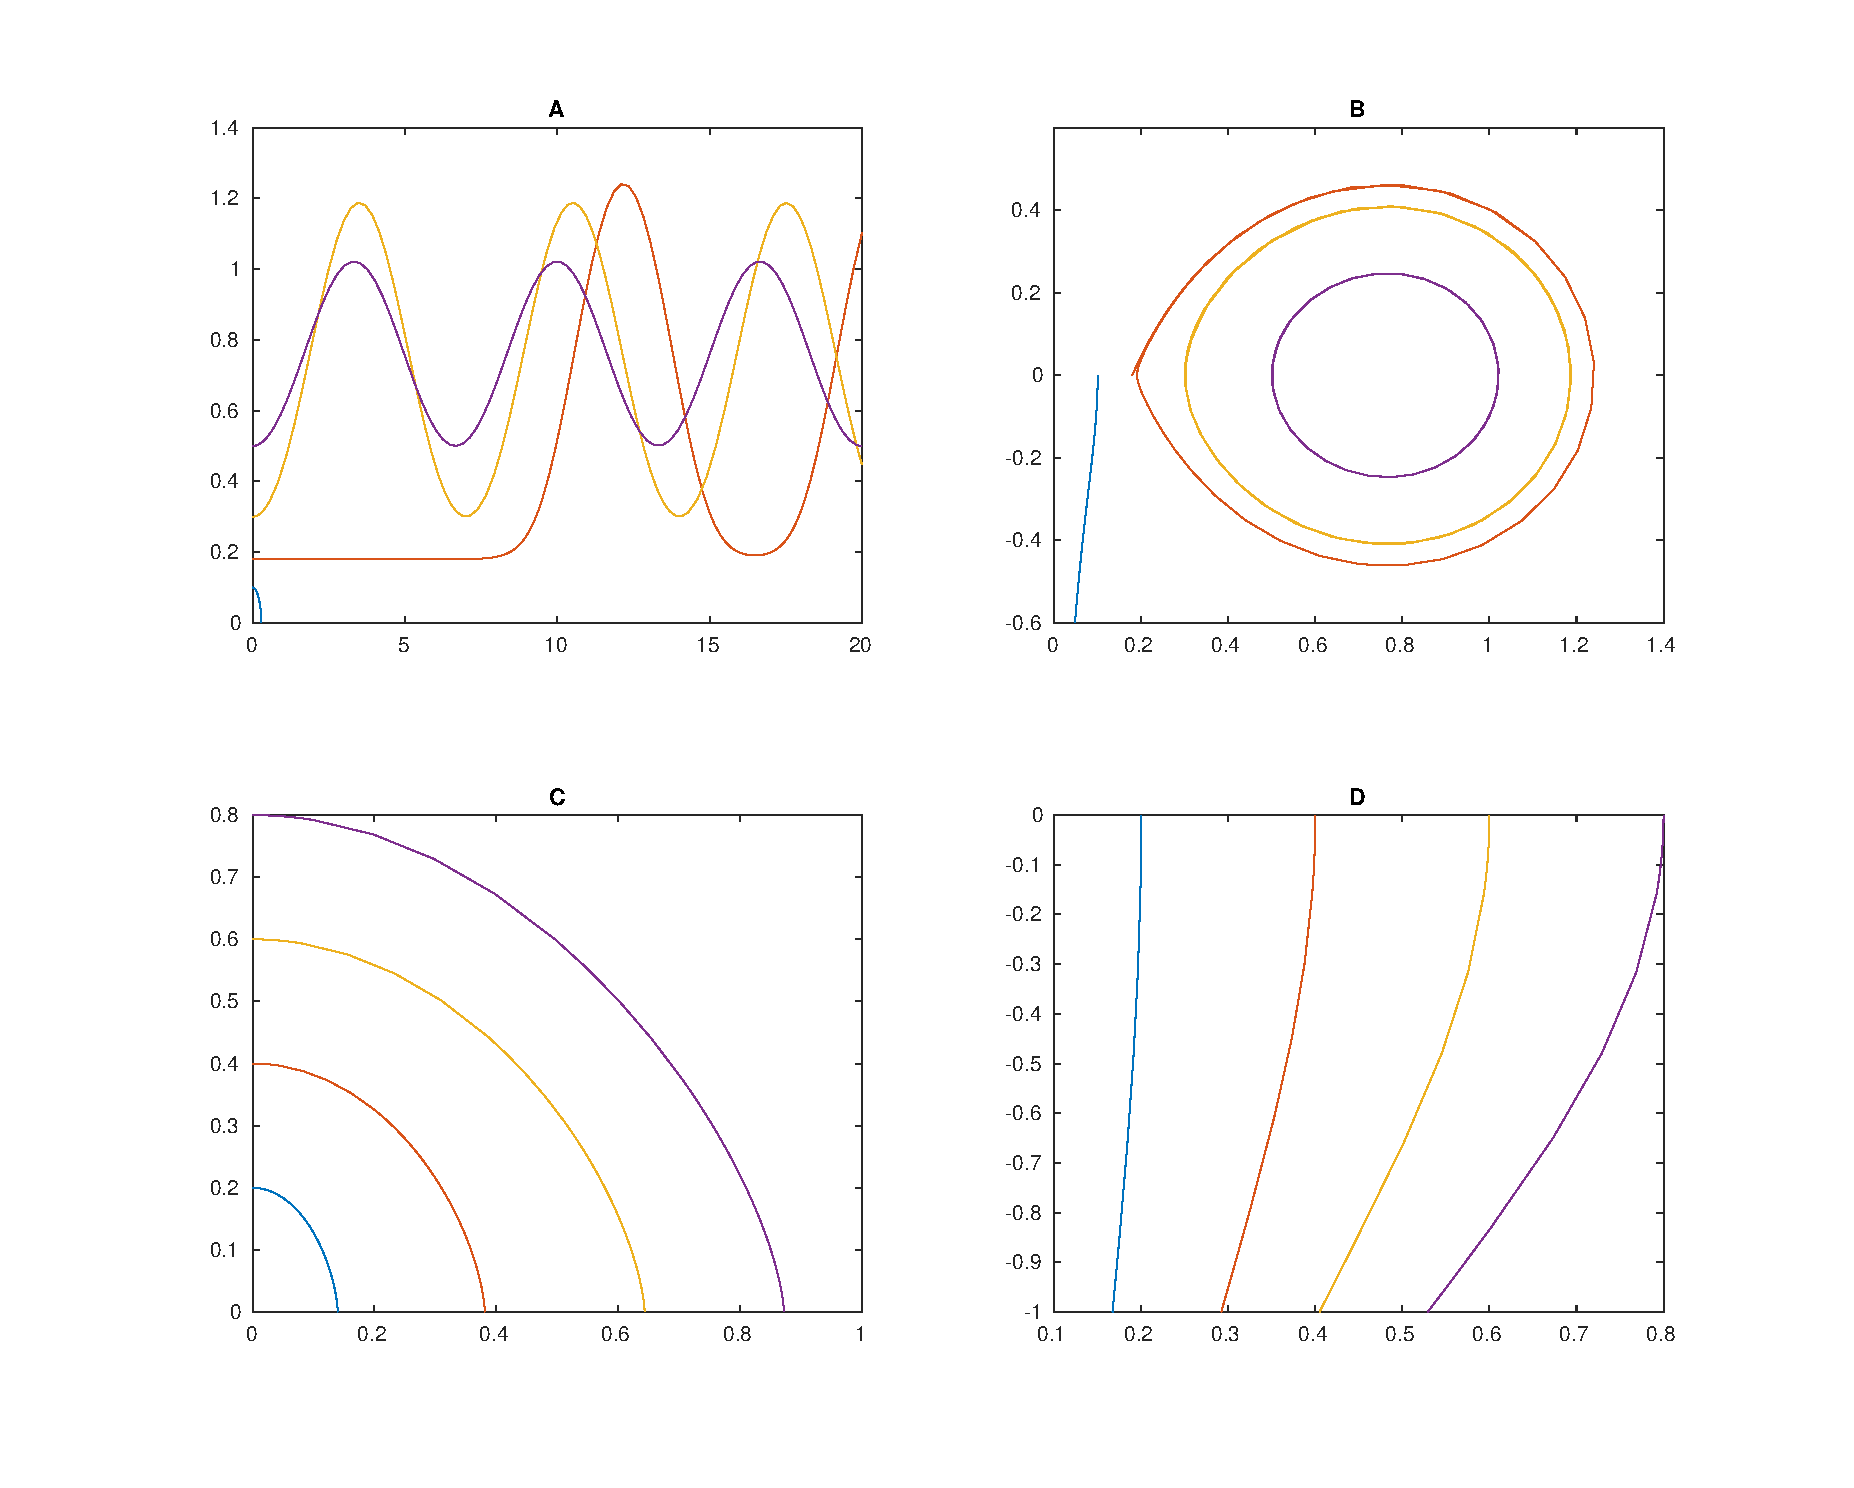
\includegraphics[width=\linewidth]{quadplot_phaseplane_versus_time_2}
    \caption{
        A comparison of plots in the traditional distance-time representation compared to in the phase portrait.
        The left column (A and C) illustrates curves as displacement against time, while the right column (B and D) draw the same plots as shown in the respective figure to the left.
        Figures in different rows show the model under different initial conditions and parameters.
        Figures A and B show the displacement $b$ with starting positions $b=0.1,~b_1,~0.3,~0.5$,
        where $b_1$ is close to the first critical point of $f$. The parameters of Equation \ref{eqn:master} are $\mu=1,~q=0.2$.
        Figures C and D are instead computed with $\mu=1,~q=1$ with $b$ taking initial values $0.2,~0.4,~0.6,~0.8$.
        In all figures, $b$ has zero initial starting velocity.
    }
    \label{fig:phaseportrait_compare}
\end{figure}

Oscillations are represented in the phase-plane as closed loops.
It becomes easier to see the critical points,
namely the stationary point in the centre of the closed loops,
and the inflection point between the regions of closure and oscillation.
See Figure \ref{fig:phaseportrait_compare} for a demonstration.

\subsection{Equations of motion represented as phase-plane curves}

Recall Equation \ref{eqn:master}, of the form $d^2b/dt^2 = f(b)$.
Assume the right hand side $f(b)$ is the derivative (with respect to $b$, remaining aware that $b$ depends on $t$) of some function $F(b)$.
Remaining aware that $b$ is a function itself of $t$, we have

\begin{equation}
    \frac{d}{db}F(b) = f(b),
\end{equation}

and if we differentiate with respect to $t$ instead, we obtain

\begin{equation}
    \frac{d}{dt}F(b) = \frac{dF}{db}\frac{db}{dt} = f(b)\frac{db}{dt}.
\end{equation}

From Equation \ref{eqn:master}, we find, on multiplying both sides by $db/dt$ and finding antiderivatives,

\begin{align}
    \frac{d^2b}{dt^2} \frac{db}{dt}                                   & = f(b) \frac{db}{dt} \\
    \Rightarrow \frac{1}{2}\frac{d}{dt}\left( \frac{db}{dt} \right)^2 & = \frac{d}{dt}F(b).
\end{align}

Integrate both sides and we obtain a result that resembles an expression for kinetic energy, namely,

\begin{equation}
    \frac{1}{2}\left(\frac{db}{dt}\right)^2 = F(b) + C,
    \label{eqn:integral_kinetic_energy}
\end{equation}

with constant of integration $C$. Variation of this constant leads to a family of solutions.
Extremely important to note is that we have an equation in terms of $\frac{db}{dt}$ and $b$, which are the vectors defining the phase portrait.
Hence the curves that appear in the phase portrait represent all the curves that appear for different $+C$.

%figure with the $P(b)$ curves matched to phase portrait curves, namely y = F(x) against 1/2 y^2 = F(x)

Notice that Equation \ref{eqn:integral_kinetic_energy} is of exactly the same form as Equation \ref{eqn:first_order_reduction},
which we derived earlier.
Both expressions represent families of curves in the phase-portrait.
However, when reducing and solving the ODE to derive the first order reduction, we made the assumption of separability of variables,
which is not true in all cases,
whereas here we have covered a different method.
In combination of results, we will want to assume

\begin{equation}
    F(b) = (1-q)b - \frac{1}{2}b^2 + \frac{\mu q^2}{2b}
    \label{eqn:integral_curve_supposed}
\end{equation}

which is not necessarily a consistent result, as discussed in the derivation, but we will use this for verification.

We can use the plots of curves defined by Equations \ref{eqn:first_order_reduction} and \ref{eqn:integral_kinetic_energy} to inspect curves in the phase portrait.
For example, we can find the particular constants $C$ such that we generate the behaviours at the critical points.

%big section here on how we can analyse the plots and zeroes of the KE curves, in order to find the requirements on f for oscillations to occur

Oscillations occur when, for some $C$, the curve $\left((db/dt)^2\right)/2 = F(b) + C$ exhibits a closed loop.
It is necessary and sufficient for there to exist a region of inflection (an interval where the derivative is positive,
elsewhere negative) in $F(b)$ in order for this to occur.
Hence the condition for oscillations to occur is equivalent to the requirement that there exists a positive \textit{region} of f(b).

Interesting behaviour occurs when the local minimum or maximum of $F(b)$ is a zero.
We want to investigate the integral curves to find the conditions required for

\begin{equation}
	F(b) + C = 0.
	\label{eqn:integral_curves_zeroes}
\end{equation}

If $\mu, q$ satisfactory for oscillations to occur,
it is evident that there exists a $C$ such that Equation \ref{eqn:integral_curves_zeroes} will have exactly two zeroes,
and the interval between these is the region in which we observe the largest oscillation.

\subsection{Matrix representation of a system of differential equations}

Recall the reduction of Equation \ref{eqn:master} to a first order system in Equation \ref{eqn:first_order_reduction}.
We will rewrite the reduction to a first order system, using the defined $f(b)$ function we are familiar with.

\begin{align}
    \frac{db}{dt}       & = \dot{b} \\
    \frac{d\dot{b}}{dt} & = f(b)
    \label{eqn:first_order_modified}   %TODO: Change variables, we don't like this it's too confusing
\end{align}

We can construct an approximation for the function $f(b)$ about a point $b_0$ using the Taylor series expansion, of the form

\begin{equation}
    f(b) = f(b_0) + (b-b_0)f'(b_0) + \frac{(b-b_0)^2 f''(b_0)}{2!} + \mathellipsis = \sum_{k=0}^\infty\frac{(b-b_0)^{k}f^{(k)}(b_0)}{k!}
    \label{eqn:taylor_series}
\end{equation}

Recall that $f(b)$ has zeroes. If we pick $b_0$ to be a zero of the function, then as $b\rightarrow b_0$,
most of the terms in the Taylor series expansion vanish\footnote{they become negligibly small}.
More precisely, since $b_0$ is a zero of $f$, the $f(b_0)$ term tends to zero.
We keep the $(b-b_0)f'(b_0)$ since, while the coefficient is small,
the terms succeeding it are far smaller in magnitude.
With the Taylor series applied, propose the approximation about a point $b_0$

\begin{align}
    \frac{db}{dt}       & = \dot{b}         \\
    \frac{d\dot{b}}{dt} & = (b-b_0)f'(b_0).
    \label{eqn:first_order_approximated}
\end{align}

Notice that this approximation is a linear system. The obtained approximation models the ODE $b''(t) = (b-b_0)(\mu q^2/b_0^3-1)$.
It is only valid local to points $b_0$ which are zeroes of $f$, so if $b-b_0$ grows in magnitude it is not sufficient.
If we suppose a substitution of the form

\begin{align}
    X & = b - b_0  \\
    Y & = \dot{b},
\end{align}

then $X$ represents the vicinity of $b$ to $b_0$, which is small,
and $Y$ is a straight substitution of the velocity value $\dot{b}$.
We can rewrite the linear system again, this time using our substituted values

\begin{align}
    \frac{dX}{dt} & = \frac{d}{dt}\left(b-b_0\right) = \dot{b} \\
    \frac{dY}{dt} & = \frac{d\dot{b}}{dt} = (b-b_0)f'(b_0)
\end{align}

which can be expressed as the matrix equation

\begin{equation}
    \frac{d}{dt}\begin{pmatrix}
        X \\
        Y
    \end{pmatrix} = \begin{bmatrix}
        0      & 1 \\
        f'(b_0) & 0
    \end{bmatrix} \begin{pmatrix}
        X \\
        Y
    \end{pmatrix}.
    \label{eqn:first_order_approximated_substituted_matrix}
\end{equation}

% discuss the implications of this analysis and the matrix eigenvectors

The implications of the matrix model allow us to perform linear system analysis local to the critical points $b_0$ satisfying $f(b_0) = 0.$
Let $\mathbf{u}=(x_i,y_i)^T$ be a vector denoting information on the plate local to $b_0$,
where $x$ is the small distance between the displacement $b$ and the critical point $b_0$,
and $y$ is the velocity of the plate.
If $u$ is an eigenvector of the matrix,
it corresponds to an eigenvalue $\lambda_i$ such that

\begin{equation}
	\frac{d}{dt} \begin{pmatrix}
		x_i \\
		y_i
	\end{pmatrix} = \lambda_i \begin{pmatrix}
	x_i \\
	y_i
\end{pmatrix},
\label{eqn:matrix_eigenvectors}
\end{equation}

implying that, if eigenpairs exist (which we can check by finding eigenvalues of the matrix),
then the eigenvectors represent change in the vicinity $\lambda_i x_i$ of the plate to the critical point,
and the change in velocity $\lambda_i y_i$ of the plate at that point.

Note that this analysis is governed by being local to the zeroes of $f(b)$.
It only provides insight on the behaviour of the model when considering these points.
When oscillations occur, it is a consequence of the condition of Equation \ref{eqn:osc_condition},
which is the condition of $f(b)$ having two positive zeroes.
Thus, the matrix equation analysis is only valid at two points,
being these solutions of $f(b)$ at the bounds of oscillation.

The eigenvectors influence motion in the vicinity of the critical points in the phase portrait.
See subfigure A of Figure \ref{fig:phaseportrait_compare}, and observe the plot which starts near the critical point.
It appears that in this case, $b$ remains stationary for a period of time before oscillations begin,
and once undergoing, the peaks of the wave are much sharper than the troughs.
This occurs because we approach the vicinity of this critical point in the phase portrait,
and Equation \ref{eqn:first_order_approximated_substituted_matrix} can be applied to find the eigenvectors.
If $\mathbf{u}$ is a vector that satisfies this equation,
then we can define points in the phase-plane that are close to these critical points by $\mathbf{u} + \mathbf{\delta u}$,
where $\delta\mathbf{u}$ is small.
Write $\mathbf{u + \delta u} = (x_i + \delta x_i, y_i + \delta y_i)^T$.
In this case, we have that

\begin{align}
    \frac{d}{dt} \begin{pmatrix}
        x_i + \delta x_i\\
        y_i + \delta y_i
    \end{pmatrix} &= \frac{d}{dt}\begin{pmatrix}
        x_i \\
        y_i
    \end{pmatrix} + \frac{d}{dt}\begin{pmatrix}
        \delta x_i \\
        \delta y_i
    \end{pmatrix} \\
    &= \lambda_i \begin{pmatrix}
        x_i \\
        y_i
    \end{pmatrix} + \begin{bmatrix}
        0 & 1 \\
        f'(b_0) & 0
    \end{bmatrix} \begin{pmatrix} % can't really do this because delta u is not necessarily an eigenvector, this needs fixing. might be able to get validity or another result out of delta u being small.
        \delta x_i \\
        \delta y_i
    \end{pmatrix} \\
    &= \lambda_i \begin{pmatrix}
        x_i \\
        y_i
    \end{pmatrix} + \begin{pmatrix}
        \delta y_i \\
        f'(b_0) \delta x_i
    \end{pmatrix}.
    \label{eqn:matrix_eigenvectors_vicinity}
\end{align}

We have assumed in Equation \ref{eqn:matrix_eigenvectors_vicinity} that $\delta u$ is not an eigenvector.
Instead we have considered only that the matrix equation holds,
since both $\delta x_i$ (the displacement of $b$ from the critical point)
and $\delta y_i$ (the velocity) are small, so we are local to the critical point on the phase-plane,
and thus can apply the matrix equation. If $\delta u$ is small, then it is negligible compared to the $\lambda_i (x_i,y_i)^T$ term.
Hence the eigenvectors influence the motion in the phase-plane local to the critical points. 

\section{Computational results provided by the single mass model}

\subsection{MATLAB results and inspection}

\begin{figure}
    \centering
    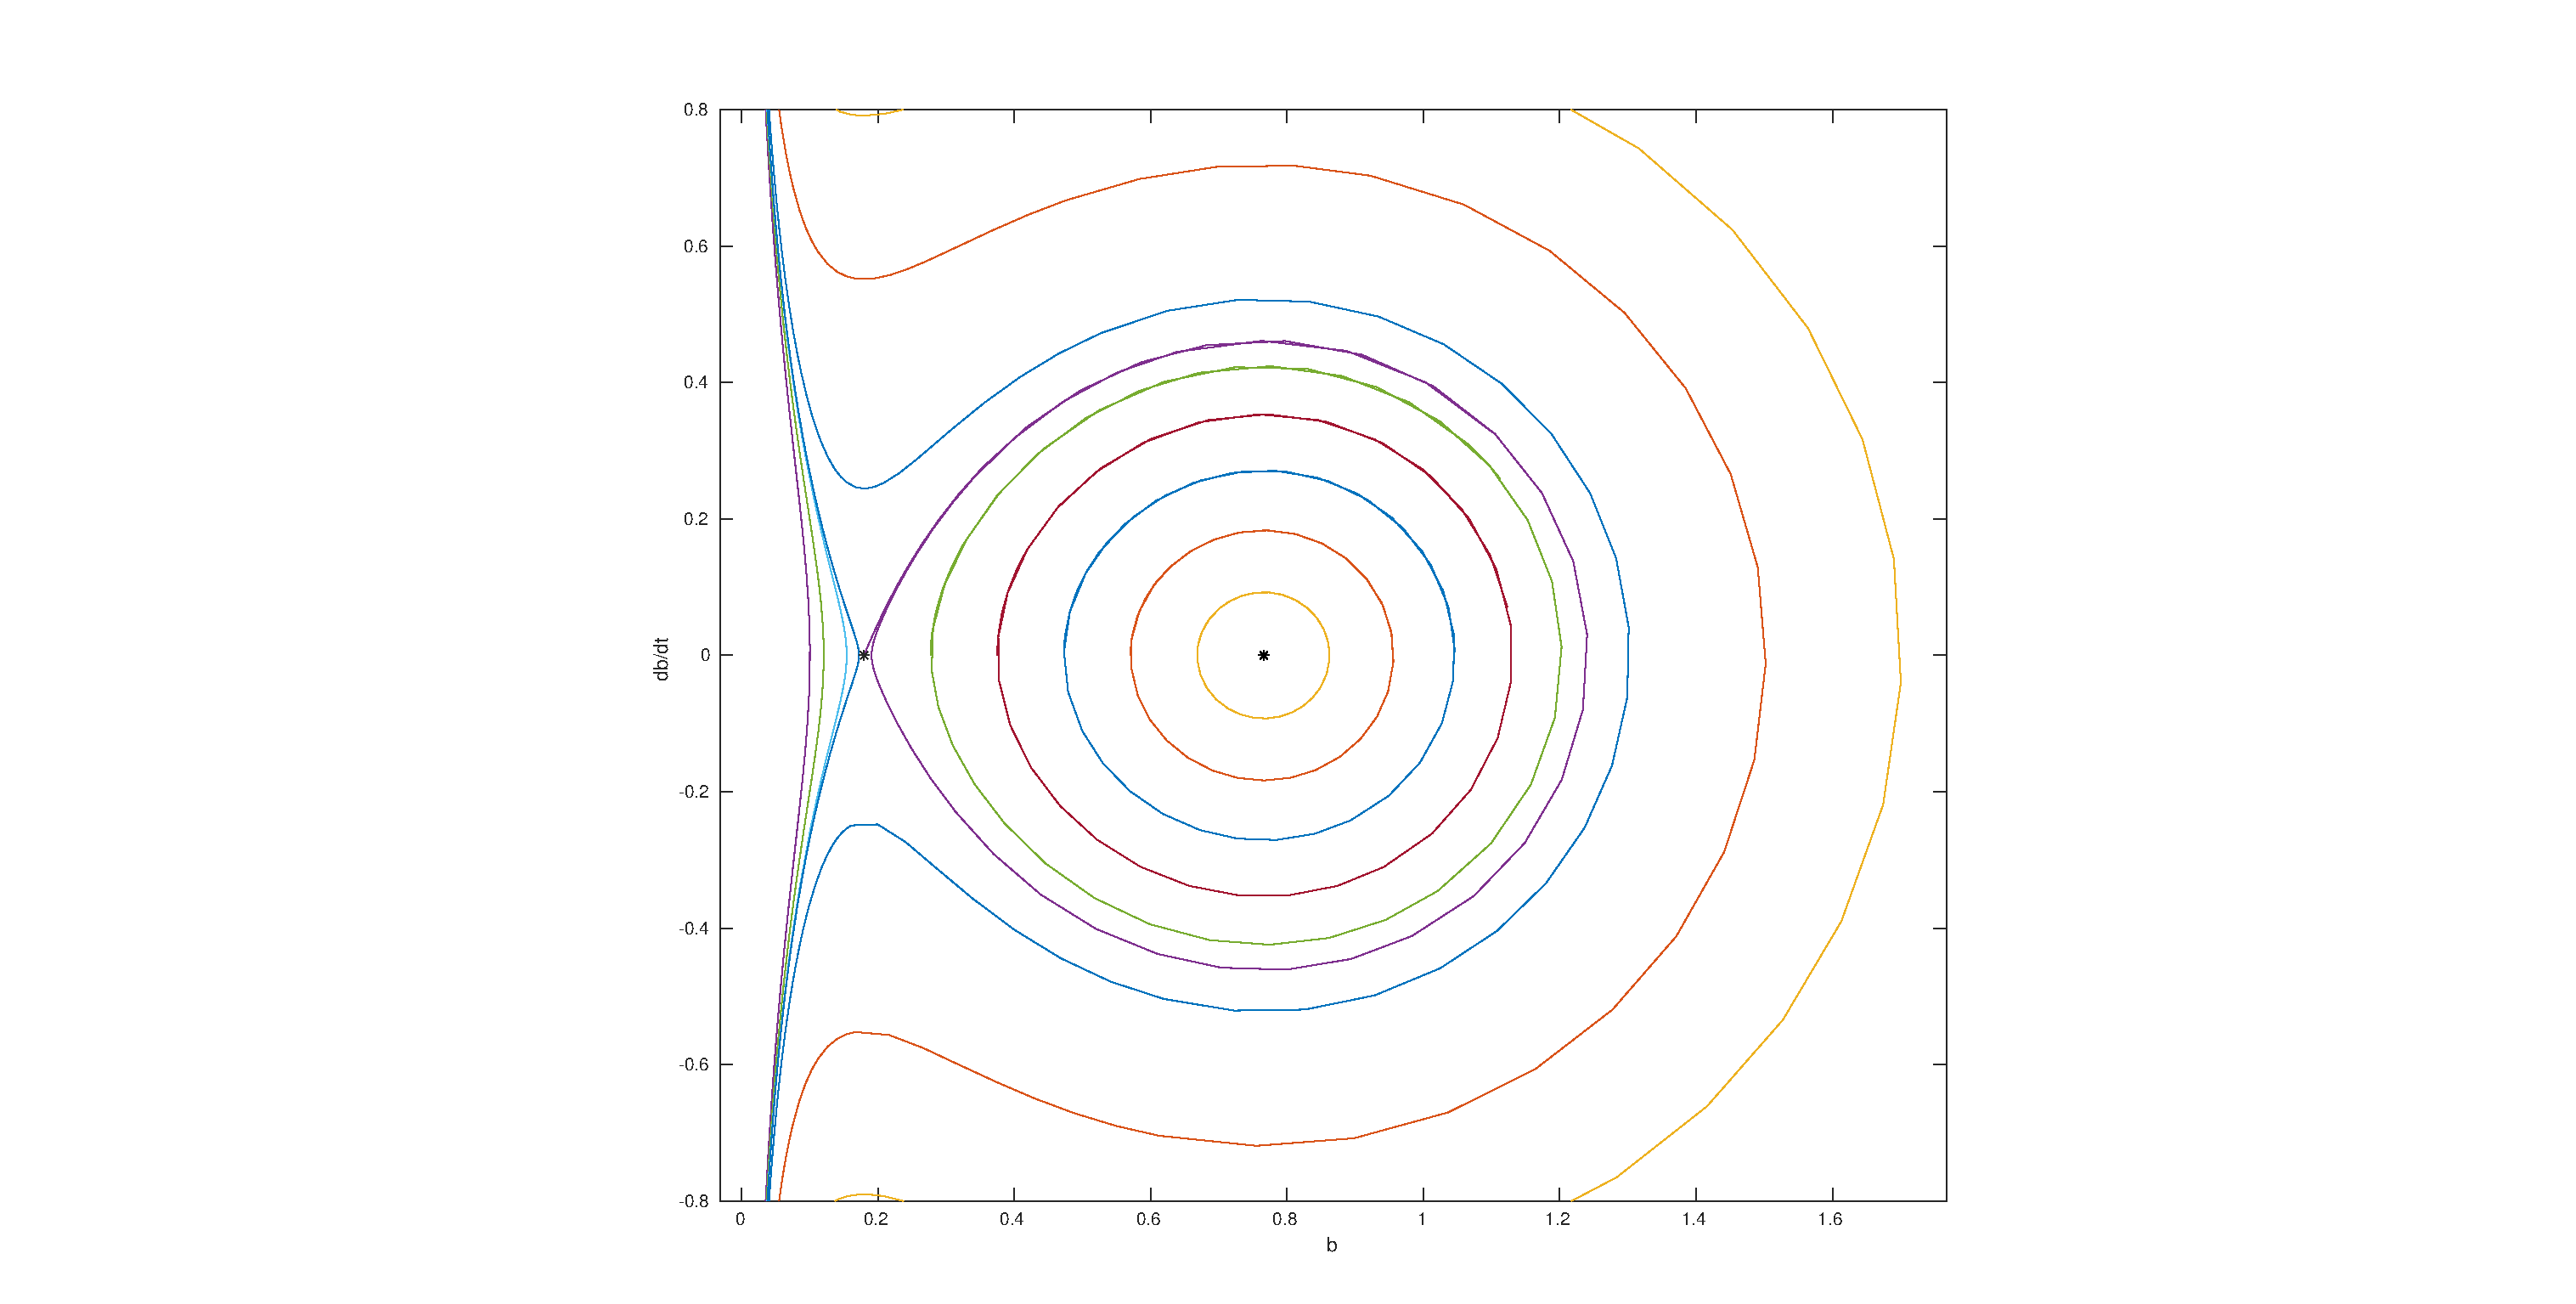
\includegraphics[width=\linewidth]{phaseportrait}
    \caption{Representation of all families of curves in the phase portrait representation of numerical solutions for Equation \ref{eqn:master}.
        The parameters are set with $\mu = 1,~q=0.2$. The critical points were computed to be $b_1 \approx 0.1795,~ b_2 \approx 0.7659$, and have been marked.
    }
    \label{fig:phaseportrait_oscillations}
\end{figure}

We will first consider a range of behaviours exhibited by the model with the fixed parameters $\mu=1, q=0.2$,
as used in sufigures A and B of Figure \ref{fig:phaseportrait_compare}.
Figure \ref{fig:phaseportrait_oscillations} is a plot showing all families of curves in the phase plane for these parameters.
%begin{dodgy}
Under the notion of topological equivalence, we can see there are four types of curve represented.
Curves that cross the horizontal axis to the left of the point $b_1$ represent the plate travelling and accelerating (negative velocity as the plate travels in the non-positive direction) immediately to closure.
Closed loops within the enclosed region are oscillations that continue indefinitely.
Curves to the right of the closed loops represent the plate also travelling towards closure,
but undergoing a period of deceleration close to the critical value.
This leaves two others. Two separate curves emerge directly from the point $b_1$ itself,
however the computation is incapable of computing this path exactly when we start at zero.
If we start at $b_1+\epsilon$ where $\epsilon$ is small,
the solution fails to form a closed loop that returns to its start,
due to the difficult behaviour of the ODE when approaching the critical point to near-exact precision.
Instead, this loop is shown to slightly increment the return position positively when an oscillation has been completed.
The stationary point at $b_2$ is the oscillation with no energy,
which is topologically equivalent to the other closed loops.
This is the oscillation with no energy,
which is topologically equivalent to all other loops. 

\subsection{Comparison to analytical results}

The region of inital $b$, with zero initial velocity, for which oscillations will occur,
is computed to be the approximate interval $(0.18,1.24)$.
We will use the supposition of Equation \ref{eqn:integral_curve_supposed}.
If the integration constant satisfies $C = -F(b_1)$,
then the curve has exactly two positive zeroes:
one being at $b=b_1$ and the other where $b>b_2$ as the curve crosses the horizontal axis as it tends to negative infinity.
Hence the range of zeroes to verify results should be the solutions to the equation $F(b)-F(b_1)=0,$ which can be written as

\begin{equation}
    (1-q)(b-b_1) +\frac{1}{2}(b_1^2-b^2) + \frac{\mu q^2}{2b} - \frac{\mu q^2}{2b_1} = 0.
    \label{eqn:integral_curves_zeroes_explicit}
\end{equation}

The value $b_1$ is, trivially, the minimal positive zero of $f(b)$ which we have already computed to be $b_1 \approx 0.18$.
We are more interested in whether or not the other end point of the interval is consistent.


% derivation of the conditions on +C which guarantee the closed orbit. 

% rigorous understanding of the range of oscillations


% behaviour of oscillations local to the "matrix points", tie in the analysis to the matrix methods.

% comparison of phaseplane and distance-time graphs




\bibliographystyle{unsrt}
\bibliography{sources}

\appendix

\section{MATLAB Scripts}

In MATLAB, we define the ODE function \texttt{OscillatorODE(t,x,q,u)} as follows:

%nicer written verbatim environment ode function here

\begin{verbatim}
function dbdt = OscillatorODE(t, x, mu, q)

b=x(1);
bdot=x(2);

dbdt=zeros(size(x));
dbdt(1) = bdot;
dbdt(2) = 1 - q - b - (mu*power(q,2))/(2*power(b,2));

end
\end{verbatim}

And it is solved with \texttt{ode45} as such:

\begin{verbatim}
q=0.1; u=1; % define fixed variables
[t, x] = ode45(@(t,x) OscillatorODE(t,x,q,u));

% distance-time plot
figure
plot(t,x(1,:))

% phase-plane plot
figure
plot(x(1,:),x(2,:))
\end{verbatim}


\end{document}

\documentclass{article}

\usepackage{amssymb}
\usepackage{amsfonts}
\usepackage{amsmath}
\usepackage{dsfont}
\usepackage{bm}
\usepackage[a4paper, total={6in,8in}]{geometry}
\usepackage{graphicx}
\usepackage{float}
\usepackage{natbib}
\usepackage{hyperref}

\graphicspath{{figures/}}

\begin{document}

\title{A Two Mass Model}
\author{Will Woolfenden}

\section{A two-mass model}

\subsection{Formulating the model}

\begin{figure}
    \centering
    \includegraphics[width=\linewidth]{twomass_bothsides.jpeg}
    \caption{General illustration of the two-mass model. Plates with mass $\mathrm{m_1},\mathrm{m_2}$ are connected to the wall of the channel by springs.
    The fluid velocity $\bm{u(x)}$ and pressure $p$ are terms we can fix local to the lung.
    The stiffness coupling between masses provides a horizontal force which we ignore by restricting the masses to one-dimensional motion along the width of the channel.}
    \label{fig:twomass_bothsides}
\end{figure}

We will begin to construct a model for phonation involving two stiffness-coupled masses.
Due to symmetry, we will only consider one side of the channel, 
We consider a steady flow $\mathbf{u}$ passing through a channel,
in which two masses cause a constriction to the fluid passage.
Each mass $m_i$ is indivually supported by a spring with Hooke constant $k_i$,
and a coupling spring with constant $k_s$ connects the two masses.

We assume the masses to move one-dimensionally, perpendicular to the principal direction of the flow,
such that they may extend indefinitely.
We make the assumption that the fluid travels similar to a plug flow approximation,
in which the fluid velocity is constant across any cross-sectional area, % citation here - there's a text "fundamentals of fluid mechanics 9780471675822"
which ignores any potential stagnation or interference.
We also neglect external forces on the fluid, such as gravity.

Air is expelled from the lung and into the upper airway, before being released into the atmosphere.
We fix a pressure $p_0$ and velocity $U_0$ local to the lung.

The formal expression for conservation of mass can be expressed as

\begin{equation}
    \iiint_V \frac{\partial\rho}{\partial t}dV = \iint_S -\rho \bm{u\cdot n}~dS,
    \label{eqn:cons_mass_formal}
\end{equation}

which can be more formally understood as the rate of change of mass over volume $V$ begin equal to the rate at which fluid is transferred over the volume's surface $S$. 
The negative term comes from the convention of using the outer unit normal of a closed surface.
We will refer to the \textit{mass flux} at $A$, denoted $Q$, being the rate at which mass of fluid is transferred over an area $A$, or formally:

\begin{equation}
    Q(x) = -\iint_A \rho \bm{u \cdot n}~dS
\end{equation}

where $x$ is the position in the dominant direction of the flow, or equivalently $x$ is in the $\mathbf{n}$ direction.
The outer unit normal $\mathbf{n}$ is the vector pointing outwards normal to any cross-sectional area. 
The integral term is negative because the outer unit normal points in the direction opposite to the flow.

\begin{figure}
    \centering
    \includegraphics[width=\linewidth]{twomass_fluxpressure.jpeg}
    \caption{The single side of the model.
    Flux $Q$ is of interest on the boundaries between masses,
    and we can use flux to either deduce or assume relationships involving pressure and fluid velocity.
    }
    \label{fig:twomass_fluxpressure}
\end{figure}

We can find the flux $Q_0$, being the flux local to the lung, from the terms $U_0,~p_0$ which are defined in our initial conditions,

\begin{equation}
    Q(x_0) = -\iint_{A_0} \rho \bm{u}(x_0)\bm{\cdot n}(x_0)~dS.
\end{equation}

Since we have a condition $u(x=x_0) = U_0$, we can write this as

\begin{equation}
    Q(x_0) = \iint_{A_0} \rho U_0~dS.
\end{equation}

We have made the assumption of incompressibility in order to write $\rho$ as a constant.
Since $A_0$ is a cross-section of known area $\mathrm{wh}$, and $U_0$ is known, we have

\begin{equation}
    Q(x_0) = \rho wh U_0
    \label{eqn:twomass_lung_flux}
\end{equation}

by evaluating the integral of a uniform quantity $U_0$ over a surface $A_0$ as the quantity multiplied by the whole area.
The flux is not uniform, because we have regions of variable volume, and a varying flux local to these regions do not break assumptions of conservation of mass.
For example, if more fluid is entering a region than what is leaving, then the volume will increase.
We have flux $Q_{in}$ on the entry border of the two mass region, and $Q_{out}$ on the exit,
with $Q_{mid}$ on the plane in between the masses.

A volume $V_i$ has dimensions $h_i \mathrm{wd}$, where $h_i + b_i = \mathrm{h}$ for $i=1,2$.
The height $h_i$ is the only parameter that may vary, since we have granted a plate with position $b_i$ one dimensional motion.
We will take time derivatives:

\begin{equation}
    \dot{V_i} = \dot{h_i} w d.
\end{equation}

Conservation of mass \ref{eqn:cons_mass_formal} in combination with incompressibility tells us that the rate of change of a volume is equal to the rate at which its enclosed mass increases.
In volume $V_1$, mass enters through flux $Q_in$ and exits through flux $Q_mid$. The case for $V_2$ is analogous.
From this we can force an assumption to relate flux around a volume to its rate of change, which can be expressed as follows:

\begin{equation}
    \begin{aligned}
        \dot{h_1} w d &= Q_\mathrm{in} - Q_\mathrm{mid} \\
        \dot{h_2} w d &= Q_\mathrm{mid} - Q_\mathrm{out}.
    \end{aligned}
    \label{eqn:twomass_flux_motion}
\end{equation}

Since the lower airway region is fixed,
the flux $Q_0$ local to the lung is equal to the flux $Q_\mathrm{in}$ on the boundary of the lower mass,
and hence it is a known term. The fluid velocity $U_\mathrm{in}$ on the flux boundary can be deduced from conservation of mass in the lower airway, i.e.

\begin{equation}
    U_\mathrm{in} = \frac{Q_\mathrm{in}}{\mathrm{w}h_1}.
    \label{eqn:twomass_flux_in}
\end{equation}

However the terms $Q_\mathrm{mid}, Q_\mathrm{out}$ are not immediately known.
We will make the assumption that the fluid velocities in the respective volumes are determined by the flux,
where we take the average of the flux on the boundaries of a region of interest:

\begin{equation}
    \begin{aligned}
        U_1 &= \frac{1}{\mathrm{w}h_1}\left(\frac{Q_\mathrm{in} + Q_\mathrm{mid}}{2}\right) \\
        U_2 &= \frac{1}{\mathrm{w}h_2}\left(\frac{Q_\mathrm{mid} + Q_\mathrm{out}}{2}\right).
        \label{eqn:twomass_velocity_interpolation}
    \end{aligned}
\end{equation}

% We want to know the values of Q_mid and Q_out so we can interpolate
% what goes in must come out.

The regions of the model which represent the upper and lower airways are rigid fixed volumes equal in cross sectional area.
If mass is conserved, then the velocity $U_0$ and flux $Q_0$ local to the lung are equal to the velocity $U_\infty$ and flux $Q_\infty$ local to the vocal opening.
Using the same method as in Equation \ref{eqn:twomass_flux_in}, we have

\begin{equation}
    U_\mathrm{out} = \frac{Q_\mathrm{out}}{\mathrm{w}h_2},
    \label{eqn:twomass_flux_out}
\end{equation}

%% weve made the firm conservation of mass argument. This may not be true if the masses are moving,
% since the volume may be increasing so more fluid goes in than comes out.
% however there is a ceiling to how much the volume can increase

where the flux $Q_\mathrm{out}$ is equal to the opening flux $Q_\mathrm{\infty}$.

We have deduced several results on the velocity of the fluid through different locations in the model,
however we don't have explicit expressions for either the plate velocities or the fluxes,
which are the key values in our statements so far.

Recall Bernoulli's equation for a steady flow.
In order to evaluate an expression for the pressure in a region,
we need to know the fluid velocity, the body forces, and the local density.
Fortunately we have assumed incompressibility, so the density $\rho$ is constant,
and we choose to neglect body forces.
Along a streamline, we have:

\begin{equation}
    \begin{aligned}
        \frac{1}{2}\rho U_0^2 + \tilde{p}_0 &= \rho\mathrm{E} &\text{(lower airway)}\\
        \frac{1}{2}\rho U_1^2 + \tilde{p}_1 &= \rho\mathrm{E} &\text{(volume $V_1$)}  \\
        \frac{1}{2}\rho U_2^2 + \tilde{p}_2 &= \rho\mathrm{E} &\text{(volume $V_2$)}  \\
        \frac{1}{2}\rho U_\infty^2 + \tilde{p}_\infty &= \rho\mathrm{E} &\text{(upper airway)},
    \end{aligned}
\end{equation}

\noindent where $\mathrm{E}$ is the Bernoulli constant on the streamline.
We will later discuss the assumption of quasisteady flow in the model,
which justifies the application of Bernoulli's equation for a steady flow.
We can rearrange and obtain explicit expressions for pressure, being

\begin{equation}
    \begin{aligned}
        \tilde{p}_0 &= \rho\left(\mathrm{E} - \frac{1}{2}U_0^2\right) \\
        \tilde{p}_1 &= \rho\left(\mathrm{E} - \frac{1}{2}U_1^2\right) \\
        \tilde{p}_2 &= \rho\left(\mathrm{E} - \frac{1}{2}U_2^2\right) \\
        \tilde{p}_\infty &= \rho\left(\mathrm{E} - \frac{1}{2}U_\infty^2\right).
    \end{aligned}
\end{equation}

In the upper airway we have $\tilde{p}_\infty$ local to the vocal opening,
hence this is \textit{atmospheric pressure}, which we will write as \(\mathrm{\tilde{p}}\).
If we have zero fluid velocity local to the lung, and the fluid is driven by the pressure,
we have that $\tilde{p}_0 = \rho \mathrm{E}$,
and if $\tilde{p}_\infty$ is atmospheric pressure, then $\rho(\mathrm{E} - U_\infty^2/2) = 0$
In combination:

\begin{equation}
    \tilde{p}_0 = \rho \mathrm{E} = \frac{\rho U_\infty^2}{2}
\end{equation}


In the regions of interest, we are concerned with the difference in pressure from atmospheric level,
which are the pressure values we actually wish to compute.
We express the pressure terms as follows:

\begin{equation}
    \begin{aligned}
        p_0 &= \rho\mathrm{E} - \rho\frac{1}{2}U_0^2 - \rho\mathrm{E} + \frac{1}{2}U_\infty^2 = \frac{1}{2}\rho\left(U_\infty^2 - U_0^2\right) \\
        p_1 &= \frac{1}{2}\rho\left(U_\infty^2 - U_1^2\right) \\
        p_2 &= \frac{1}{2}\rho\left(U_\infty^2 - U_2^2\right).
    \end{aligned}
\end{equation}

\noindent Importantly \(p_0 = \tilde{p}_0\) is still the forcing term.

%now we're really in a pickle. How can we have atmospheric pressure when we can force pressure?

We now impose the assumtion of a quasisteady flow.
This lets us regard a consistent flux $Q$ throughout the mechanics,
rather than separate fluxes at different regions of interest.
Equations \ref{eqn:twomass_flux_in}, \ref{eqn:twomass_flux_out} give us an expression for velocity in terms of flux and the channel dimensions,
which we can generalise outside the region of interest:

\begin{equation}
    U = \frac{Q}{\mathrm{wh}},
\end{equation}

\noindent and in a region of interest we use the variable channel height instead

\begin{equation}
    U_i = \frac{Q}{\mathrm{w}h_i}
\end{equation}

\noindent for \(i=1,2\).

We now have a construction for pressure in terms of the plate displacement, thus can write the pressure-induced force on the plate.
Given \(i=1,2:\)

\begin{equation}
    \begin{aligned}
        p_i &= \rho\left(\mathrm{E} - \frac{1}{2}U_i^2 \right) \\
        &= \frac{1}{2}\rho\left(U_\infty^2 - U_i^2\right) \\
        &= \frac{1}{2}\rho\left( \left(\frac{Q}{\mathrm{wh}}\right)^2 - \left(\frac{Q}{\mathrm{w}h_i}\right)^2 \right) \\
        &= \frac{\rho Q^2}{\mathrm{w}^2}\left( \frac{1}{\mathrm{h}^2} - \frac{1}{h_i^2} \right)
    \end{aligned}
    \label{eqn:twomass_pressureterm}
\end{equation}

\begin{figure}
    \centering
    \includegraphics[width=\linewidth]{twomass_springs.jpeg}
    \caption
    {
        Illustration of the lengths $b_1,b_2$ and the springs connected to the masses.
        The springs connected to the wall act as support,
        preventing the Bernoulli pressure drop from forcing the walls into closure similarly to the single mass model.
        The coupling spring provides a stiffness such that the two masses can be thought of as one body consisting of two components.
        The springs allow us to deduce forces acting on the masses which stimulate motion by Newton's second law. 
    }
    \label{fig:twomass_springs}
\end{figure}

We use linear elastic Hooke springs to model the stiffness of the walls.
Support springs are similar to the original model we have considered,
however we now introduce stiffness coupling between two separate walls.
A plate $i = 1,2$ is connected to the wall by a stiffness spring with constant ${k}_i$.
The coupling spring has constant $\mathrm{k}_s$, and the resting equilibrium positions of all springs are at $0$.

The forces on a plate with position $b_i$ provide the equation of motion by Newton's second law:

\begin{equation}
    \mathrm{m}_i\frac{\mathrm{d}^2 b_i}{\mathrm{d}t^2} = -F_\mathrm{stiffness} - F_\mathrm{pressure} + F_\mathrm{coupling}
\end{equation}

\noindent for $i=1,2$. In full:

\begin{equation}
    \begin{aligned}
        \mathrm{m}_1\frac{\mathrm{d}^2 b_1}{\mathrm{d}t^2} &= -\mathrm{k}_1(b_1 - \mathrm{b}*) - \frac{wd\rho Q^2}{w^2}\left(\frac{1}{\mathrm{h}^2} - \frac{1}{(\mathrm{h}-b_1)^2} \right) + \mathrm{k}_s(b_2-b_1) \\
        \mathrm{m}_2\frac{\mathrm{d}^2 b_2}{\mathrm{d}t^2} &= -\mathrm{k}_1(b_2 - \mathrm{b}*) - \frac{wd\rho Q^2}{w^2}\left(\frac{1}{\mathrm{h}^2} - \frac{1}{(\mathrm{h}-b_2)^2} \right) + \mathrm{k}_s(b_1-b_2)
    \end{aligned}
\end{equation}

\noindent where $b*$ is the resting position of both masses. It will be easier to make $h$ the variable of interest, since closure at $h=0$ is identifiable,
and we will impose the resting position to be $h* = \mathrm{h}$. Recall the definition $b_i + h_i = \mathrm{h}$. The conversion yields

\begin{equation}
    \begin{aligned}
        \mathrm{m}_1\frac{\mathrm{d}^2 h_1}{\mathrm{d}t^2} &= -\mathrm{k}_1(h_1 - \mathrm{h}) + \frac{wd\rho Q^2}{w^2}\left(\frac{1}{\mathrm{h}^2} - \frac{1}{h_1^2} \right) + \mathrm{k}_s(h_2-h_1) \\
        \mathrm{m}_2\frac{\mathrm{d}^2 h_2}{\mathrm{d}t^2} &= -\mathrm{k}_2(h_2 - \mathrm{h}) + \frac{wd\rho Q^2}{w^2}\left(\frac{1}{\mathrm{h}^2} - \frac{1}{h_2^2} \right) + \mathrm{k}_s(h_1-h_2).
    \end{aligned}
\end{equation}

We introduce the following parameters

\begin{equation*}
    \begin{aligned}
        h_1 = \mathrm{h}\tilde{h}_1,~h_2 = \mathrm{h}\tilde{h}_2,~t=\sqrt{\frac{\mathrm{m}_1}{\mathrm{k}_1}}\tilde{t}, \\
        \alpha = \frac{\mathrm{m}_2}{\mathrm{m}_1},~\lambda = \frac{\mathrm{k}_2}{\mathrm{k}_1},~\omega = \frac{\mathrm{k}_s}{\mathrm{k}_1} \\
        \beta = \frac{\mathrm{wd}\rho U_\infty^2}{2\mathrm{k}_1\mathrm{h}}
    \end{aligned}
\end{equation*}

and the coupled fourth-order system of differential equations can be reduced to the nondimensional problem:

\begin{equation}
    \begin{aligned}
        \frac{\mathrm{d}^2 \tilde{h}_1}{\mathrm{d}\tilde{t}^2} &= 1 - \tilde{h}_1 + \beta \left( 1 - \frac{1}{\tilde{h}_1^2} \right) + \omega(\tilde{h}_2-\tilde{h}_1) \\
        \alpha\frac{\mathrm{d}^2 \tilde{h}_2}{\mathrm{d}\tilde{t}^2} &= \lambda(1 - \tilde{h}_2) + \beta \left( 1 - \frac{1}{\tilde{h}_2^2} \right) + \omega(\tilde{h}_1-\tilde{h}_2).
    \end{aligned}
    \label{eqn:twomass_coupled_system}
\end{equation}

The two mass generalises the concepts from the original model we investigated,
and maintains a lot of important features.
Before investigating the behaviour of the coupled system of equations,
we will verify that the new model can reproduce behaviours we have already seen.
Namely, if we were to configure the problem as two equal masses with the same stiffness,
and a strong coupling between them,
then we would expect the oscillating behaviour of the original model to be replicated.
We will then reduce the stiffness coupling and introduce different lateral stiffnesses for each mass,
investigating how the oscillating components affect one another in a coupled system.
Finally if we reduce the coupling to a negligible amount,
we would then expect the masses to behave near independently.

\subsection{Strong coupling}

We study the behaviour of two strongly coupled masses of equal stiffness, represented by \( \alpha = 1,~\lambda = 1,~\omega \gggtr 1\).
The coupled system of equations in \ref{eqn:twomass_coupled_system} take the same form for each.
Similarly to the single-mass model, we can use the existence of stationary equilibria to determine the potential for oscillations to occur.
Imposing the existence of a stationary equilibrium solution \(h_1 = h_2 = x\) imposes that
\begin{equation}
    1 - x + \beta\left(
        1 - \frac{1}{x^2}
    \right) = 0,
\end{equation}
where the coupling term cancels.
The stable equilibria exist at the positive zeroes of the function we define:
\begin{equation}
    f(h) = 1 - h + \beta \left( 1 - \frac{1}{h^2} \right).
    \label{eqn:twomass_existence_of_equilibria}
\end{equation}
Existence of zeroes is equivalent to the local maximum, beloning at \(h = \left( 2\beta \right)^{1/3}\) being positive-valued such that the zeroes exist,
which can be written as

\begin{equation}
    1 - \left(2\beta\right)^\frac{1}{3} + \beta\left( 1 - (2\beta)^\frac{-2}{3} \right) \ge 0,
    \label{eqn:twomass_zeroes_equal_stiffness}
\end{equation}
with equality if there is only one equilibrium solution.
Equation \ref{eqn:twomass_zeroes_equal_stiffness} reduces to
\begin{equation}
    \frac{(1+\beta)^3}{\beta} \ge \frac{27}{4}.
\end{equation}
This is satisfied for all positive $\beta>0$ and has equality at $\beta = 0.5$.
If the initial conditions for \(h_1, h_2\) set their individual positions between the two equilibrium solutions,
provided they exist,
then we observe coupled oscillations as in Figure \ref{fig:twomass_dominant_osc}.
\begin{figure}
    \centering
    \includegraphics[width=\linewidth]{figures/twomass_equal_coupleosc.eps}
    \caption{Coupled oscillations under parameters \((1, 1, 3, 20)\) and initial conditions \(h_1 = 1.2, h_2 = 3.59\),
    with equilibrium positions \(1\) and \(3.7913\). The pair of masses, forced into different initial positions,
    equioscillate about each other rapidly, while following a dominant oscillation path.}
    \label{fig:twomass_dominant_osc}
\end{figure}

An important feature is that for \(\lambda = 1\), there exists a stationary stable equilibrium solution.
We will see later that this case is not satisfied elsewhere. %or is it

\begin{figure}
    \centering
    \includegraphics[width=0.75\linewidth]{twomass_coupling_pillowplot}
    \caption{
        Plot of opposing displacements ($h_2$ against $h_1$). The motion is constrained within a fixed region,
        however it is quasiperiodic since the oscillations will, given infinite time, fill the entire illustrated area.
        Important parameters are \(\omega = 10, \lambda = 0.8\) so the stiffnesses are not equal and the masses are strongly constrained together.
    }
    \label{fig:twomass_quasiperiodic}
\end{figure} %MOVE THIS!!!!!

The equilibria, being the solutions of Equation \ref{eqn:twomass_existence_of_equilibria}, are identical for both components of the system of differential equations,
provided the parameters satisfy \(\alpha = 1, \lambda = 1, \omega \gggtr 1\) in order to model two strongly coupled masses.
This allows us to discuss the solutions to a single equation without loss of generality.
Assuming there exist equilibria \(x\), 
we can construct the Jacobian and determine the stability local to these equilibria.
We regard the whole system with the variable \(h_1=h_2=h\).
The system of derivatives in the single case can be written as

\begin{equation}
    \begin{aligned}
        \frac{\mathrm{d}h}{\mathrm{d}t} &= g \\
        \frac{\mathrm{d}g}{\mathrm{d}t} &= f(h) = 1-h +\beta\left(1-\frac{1}{h^2}\right),
    \end{aligned}
\end{equation}
which vectorises as

\begin{equation}
    \frac{\mathrm{d}}{\mathrm{d}t} \begin{pmatrix}
        h \\
        g
    \end{pmatrix} = \begin{pmatrix}
        g \\
        f(h)
    \end{pmatrix}.
\end{equation}
Recall we have stationary equilibria which we call \(x\). Compute the taylor series of \(f(h)\) local to this point.

\begin{equation}
    f(h) = f(x) + (h-x)f'(x) + (h-x)^2\frac{f''(x)}{2!} + \mathellipsis =\sum_{0}^{\infty} (h-x)^n\frac{f^{(n)}(x)}{n!}.
\end{equation}
Similarly to our earlier reasoning, we truncate the Taylor series to the approximation $f(h) \approx (h-x)f'(x)$.
The vectorised approximation becomes

\begin{equation}
    \frac{\mathrm{d}}{\mathrm{d}t}\begin{pmatrix}
        h \\
        g
    \end{pmatrix} = \begin{pmatrix}
        g \\
        (h-x)f'(x)
    \end{pmatrix}.
\end{equation}
Substituting \(U = h-x\) and \(V = g\) we obtain

\begin{equation}
    \frac{\mathrm{d}}{\mathrm{d}t} \begin{pmatrix}
        U \\
        V
    \end{pmatrix} = \begin{bmatrix}
        0 & 1 \\
        f'(x) & 0
    \end{bmatrix} \begin{pmatrix}
        U \\
        V
    \end{pmatrix} 
\end{equation}
We can inspect the eigenvalues of this matrix to determine the stability of the equilibrium solutions. %so do it
Coming from the original model, we would expect three cases in which we can analyse equilibria, being

%EIGENVALUES HERE PLEASE

\begin{enumerate}
    \item There are no equilibrium solutions and oscillations never occur,
    \item There is one equilibrium solution and oscillations do not occur,
    \item There are two equilibrium solutions and oscillations may occur about a stable stationary point.
\end{enumerate} %more on this

The cases in this model are reduced, since the stationary point $1$ is always a solution for any value of \(\beta\).
Hence there can either be $1$ or $2$ stationary points.
The single solution exists in the case of equality in Equation \ref{eqn:twomass_zeroes_equal_stiffness}.


%it gets rough from here

\subsection{Weak coupling}

\begin{figure}
    \centering
    \includegraphics[width=\linewidth]{twomass_individual_converging}
    \caption{
        Parameters given are \((1, 0.8, 3, 1)\). The masses oscillate near independently starting at different positions $(1.96, 0.83)$ at time $t=0$.
        The figures, left to right, progressively increase the time we run the computation.
        We can see in the left-most plot that the weak coupling leads to the masses oscillating at independent frequencies.
        As running time increases, the masses converge to their own equilibrium positions.
        }
    \label{fig:twomass_independent}
\end{figure}
We now develop our analysis of the two mass model by examining multiple dimensions of the parameter space.
First, we will retain the stiffness coupling \(\omega \gggtr 1\),
but consider the cases induced by \(\lambda \ne 1\), which are where the relative stiffnesses for each component are not the same.
We freely change \(\beta\) since it is similar to a forcing term, which we can change to observe different behaviours of the model.

If we impose \(\omega \llless 1\), we expect both masses to act near independently.
We can see in figure \ref{fig:twomass_independent} that this is mostly the case, since oscillations occur with apparent independence.
However the oscillations converge, gradually decreasing in amplitude and increasing in wavelength.


\subsection{Intermediate coupling force}

In general, we observe quasiperiodic oscillating motion of the masses.
We can break the behaviours down into three distinct categories, being
\begin{enumerate}
    \item oscillating indefinitely,
    \item stationary equilibrium,
    \item closure.
\end{enumerate} 
Figure \ref{fig:twomass_quasiperiodic} demonstrates the indefinite oscillations. 
The borders of the shape accommodate the restrictions of the coupling force,
and the individual stiffness of the masses.


We consider the equilibria instead to be the solutions of two equations for each component, being:

\begin{equation}
    \begin{aligned}
        \hat{f}_1(h) &= 1 - h + \beta\left( 1-\frac{1}{h^2} \right) &= 0 \\
        \hat{f}_2(h) &= \lambda(1-h) + \beta\left( 1-\frac{1}{h^2} \right) &= 0.
    \end{aligned}
    \label{eqn:twomass_coupled_equilibria_uncoupled}
\end{equation}
The existence of equilibrium solutions is determined by two assumptions, being
\begin{align*}
    f_1 \left( (2\beta)^\frac{1}{3} \right) &\ge 0, \\
    f_2 \left( \left( \frac{2\beta}{\lambda} \right)^\frac{1}{3} \right) &\ge 0,
\end{align*}
where if both are satisfied, then each mass has two points in space where it belongs to a state of stationary equilibrium.
It is important to note the assumption that \(h_1=h_2\) which we made when exploring earlier cases,
which is no longer a valid assumption to make. 
Therefore, we cannot neglect the stiffness coupling term,
which makes it much harder to determine potential points of equilibrium of the system.
We will refer to the solutions of Equation \ref{eqn:twomass_coupled_equilibria_uncoupled} as the \textit{particular equilibria},
while the actual solutions to the coupled equations will be referred to as the \textit{general equilibria}.
If we are to define the properties of stationary equilibria more rigorously,
we will be able to understand the properties of the model better.
We want all equilibrium solutions \(h-1 = x, h_2 = y\) which solve the coupled differential equations.
These general equilibria are defined as the zeroes of the functions
\begin{equation}
    \begin{aligned}
        f_1(x) &= 1-x + \beta\left(1 - \frac{1}{x^2}\right) + \omega(y-x) \\
        f_2(y) &= \lambda(1-y) + \beta\left(1 - \frac{1}{y^2}\right) + \omega(x-y).
    \end{aligned}
\end{equation}
Unlike before, an equilibrium solution is a pair \((x,y)\) which solve both equations,
thus the problem can be reduced to
\begin{equation}
    1-x + \beta\left(1 - \frac{1}{x^2}\right) + \omega(y-x) = \lambda(1-y) + \beta\left(1 - \frac{1}{y^2}\right) + \omega(x-y) = 0.
    \label{eqn:twomass_noalpha_equilibrium_solutions}
\end{equation}
Our solutions are determined by one equation involving three parameters \((\lambda, \beta, \omega)\), which we want to solve for two variables \((x,y)\).
This is a challenge to solve, but to start we know from the formulation of the model and the nondimensionalisation that \((x,y) = (1,1)\) is an equilibrium solution for all values of the parameters.
Solutions are found by computation via. Newton's method.
\begin{figure}
    \centering
    \includegraphics[width=\linewidth]{twomass_families_equilibria}
    \caption{
        Curves A (left), B(middle), C (right), representing the equilibrium solutions to the coupled equations under separate parameters.
        The $x$ and $y$ axes are the equilibrium solutions of $f_1 = 0$ and $f_2=0$ respectively. 
        In all graphs, the blue curve is the family of all equilibrium solutions for $x$,
        the red curve is the family of solutions for $y$,
        and the green line is the line $y=x$.
        Curves A, B and C all feature parameters \(\alpha = 1,~\lambda=0.8,~\omega = 0.5\), changing $\beta$,
        where \(\beta_\mathrm{A} = 4,~\beta_\mathrm{B} = 2,~\beta_\mathrm{C} = 0.8\)
        The red and blue curves intersect at points $f_1=f_2=0$,
        which are equilibrium solutions satisfying both equations.
        The points at which a curve intersects the $y=x$ line are the points that satisfy equilibrium of that equation, and also satisfy $y=x$,
        which cancels the coupling term.
        These are the solutions of $\hat{f_1}=\hat{f_2}=0$ which we covered earlier.
    }
    \label{fig:twomass_equilibrium_curves}
\end{figure}
Figure \ref{fig:twomass_equilibrium_curves} visualises the families of solutions to the equations.
The iterative method starts by using Newton's method to solve the separated equations, negligent of the stiffness coupling.
These individual stationary points are used for a second implementation of Newton's method solving a homogeneous equation of a vector function \(F = [f_1, f_2]^\mathrm{T}\).
This computes an equilibrium pair \(x,y\), which solves the coupled equations. % IT TOOK 2 DAYS
In most cases, there are four individual equilibrium solution pairs to the coupled equations,
being the intersection points of the hyperbolas in Figure \ref{fig:twomass_equilibrium_curves}.
We will refer to the solution pairs close to the line $y=x$ as the \textit{diagonal equilibria},
and the other solutions as the \textit{off-diagonal equilibria}.
On inspection, as the extrema of the curves approach each other,
the off-diagonal equilibria annihilate.







\end{document}



\chapter{Critique of the models, overview of results and conclusion}
\label{cha:conclusion}

\section{Improving our models}

\subsection{Energy}

Both the single mass and the two mass model are systems which perfectly preserve energy.
This is not consistent in the computations,
but we have shown for both models that there exists a constant term,
depending on the variables of position and velocity,
which is unchanging in time.
From a realistic perspective,
systems tend to dissipate energy and eventually come to rest,
rather than behaving like perfect conservative machines that operate indefinitely.

Both models we have studied lack any form of damping,
so all potential energies are perfectly transferred to kinetic energies and vice versa.
If we were to introduce a damping parameter,
we would observe closed oscillations about a stationary point to always converge to that equilibrium,
rather than oscillating indefinitely.

A mass $m$ attached to a Hooke spring obeys the ODE
\begin{equation*}
	m\frac{\mathrm{d}^2 x}{\mathrm{d}t^2} + k(x-x_0) = 0
\end{equation*}
where $x$ is the length of the spring, $x_0$ is the length at rest,
$k$ is the stiffness,
and $t$ is time.
This is the equation for a simple harmonic oscillator,
with equilibrium solution $x=x_0$.
The general solution is the expression
\begin{equation*}
	x = x_0 + A\exp \left(
		\sqrt{-\frac{k}{m}}t
	\right) + B\exp \left(
		-\sqrt{-\frac{k}{m}}t
	\right),
\end{equation*}
where $A$ and $B$ are free constants.
With the inclusion of a damping parameter,
we obtain a different ODE
\begin{equation*}
	m\frac{\mathrm{d}^2 x}{\mathrm{d}t^2} + c\frac{\mathrm{d}x}{\mathrm{d}t} + k(x-x_0) = 0
\end{equation*}
where the constant $c$ describes the damping strength.
We retain the equilibrium solution $x=x_0$, but the general solution changes to
\begin{equation*}
	x = x_0 + A \exp \left(
		\frac{-c+\sqrt{c^2-4mk}}{2m}t
	\right) + B \exp \left(
		\frac{-c-\sqrt{c^2-4mk}}{2m}t
	\right).
\end{equation*}
We require $m,~k,~c$ to be positive constants.
The harmonic oscillator is periodic,
whereas the damped harmonic oscillator eventually decays to rest at the equilibrium.

Our models describe systems where energy is perfectly transferred between useful forms,
namely potential and kinetic energies.
In other words, the systems we study have $100\%$ efficiency.
In reality, there are virtually no dynamical systems with this level of efficiency,
rather that some energy is always wasted.
If would be interesting to develop our models by introducing forms of energy dissipation,
such that our models would not describe systems which are $100\%$ efficient.
We could then consider how the forcing pressure could adapt to continue phonation to take place when the motion of the vocal cords begins to decay towards equilibrium.

% talk about voice and natural systems that lose energy

\subsection{Elasticity}

From studies into the material properties of the vocal cords,
they have been observed to deform under stress with nonlinear elasticity \cite{alipour_2012}.
However, in the models we have studied,
the stiffness of the vocal cords are modelled with linear elasticity by a Hooke spring.
It is important to note that in the two mass model,
we simplified these assumptions further,
by approximating the stiffness coupling by a linear force,
rather than as the vertical component of a diagonal spring.

The purpose of our mathematical models are to describe the potentially intricate motion of the vocal cords.
In order to do this,
we used Hooke springs to model the stiffnesses.
While not ideal, these are fundamental to the quasiperiodic behaviours we observed in the two mass model.
If we considered non-linear stiffnesses,
these might provide fundamentally different oscillations to our observations.
However, our analysis does not extend to the impacts of different spring behaviours on the results.
Rather, we made the approximation of linear Hooke springs and analysed their impact in depth.

It also serves to mention that the linear Hooke spring is a first-order approximation to the stiffness of a real spring.
As such, it is reasonably accurate for small displacements,
which occur in the proximity of stable equilibria,
being a large portion of our analysis.

\subsection{Stablility of fluid flow}

In both models,
we applied Bernoulli's equation for a steady flow in order to deduce a relationship between the velocity and the pressure of the fluid.
It is possible for the spoken sounds in phonation to be produced by a steady flow,
but phonation can occur more generally for unsteady, turbulent flows,
and this is not a case which is accommodated in our modelling.

In the two mass model,
we forced the assumption of a quasisteady flow,
however this reduced the cases we accommodated in the modelling.
Ideally we would construct a model which provides accurate simulation of vocal folds moving, subject to a turbulent flow through the glottis.
However, the quasisteady flow still provided rich results which led to a wide variety of behaviours which we were able to analyse.
Were we to develop the model and introduce the non-steady flow,
it would be very important to replicate results from the quasisteady flow assumption.
This is because if a model cannot retain a result when a component changes,
then there may be something fundamental to that original component,
which we have now lost.
As such,
it was important to focus on the quasisteady flow assumption,
even if this does not capture the range of flow types that may be involved in phonation.

When we began to discuss the two mass model,
we introduced relationships between the fluxes and the velocities of the masses.
We supported these suggestions with the argument of conservation of mass for an incompressible fluid.
However, the quasisteady flow was a stronger assumption which neglected these rules.
If we were to develop the model,
these assumptions on the flux would be good candidates to involve in the modelling.
The quasisteady flow implies ``$\mathrm{change~in~volume}=\mathrm{change~in~flux}$'' for any fixed volume.

\subsection{Physical structure of the model}

The formulation of the two mass model involved extremely simple geometry,
being the flow through a rectangular channel.
A more varied and irregular structure,
similar to the interior shape of the larnyx and glottis,
could potentially influence the dynamics of the fluid flow.
A varying inner channel width could have implications in Bernoulli flow,
and could contribute to more complex flow patterns in phonation.

The masses which model the vocal cord are extremely simple objects,
being stiffness-coupled planes,
and are restricted to one dimensional motion in the direction of their ourward normal.
In reality, the vocal folds have a much more intricate shape than the cuboid blocks we modelled them as.
We could develop the two mass model by constructing the vocal fold with a much more gemoetrically complex shape,
and allowing more degrees of freedom in their motion.
This would lead to more complex behaviour in the motion of the masses,
but it would be difficult to recover results from the simpler model which we have analysed.
This is because the ODE we have analysed in the two mass model is characteristic of the one dimensional motion.
If we were to remove this restriction,
we would obtain a system of PDEs describing motion in more than one degree of freedom,
and it would be difficult to replicate the one dimensional results from our two mass model.

\section{Discussion}

\subsection{Aims}
% what did we aim to do

In this project,
we aimed to explore mathematical models for phonation,
and analyse the characteristics that they can produce.
We began by exploring a single mass model from a research paper,
and derived results on its behaviour.
We explored equilibrium solutions and criteria for closure.

We generalised the properties of the single mass problem into a model involving two separate, stiffness-coupled masses.
We analysed distinct behaviours of the two mass model,
again investigating equilibrium solutions.
We investigated the complex shape of the motion of the masses,
and performed computational Fourier analysis on different results to provide insight into the frequencies of the oscillations.

\subsection{The single mass model}
% what does the single model do

The single mass model exhibits oscillations when parameters take suitable values.
Orbits oscillate about a stable equilibrium $b_2$ in the phase portrait.
In the proximity of the unstable equilibrium $b_1$,
orbits will gravitate towards the unstable point.
Trajectories near $b_1$ outside the bound for oscillations will diverge from this unstable point and eventually reach closure.

\subsection{The two mass model}
% what does the two mass model do

We constructed the two mass model by generalising the single mass model,
but we chose to cover the formulation of the model from scratch.
Two masses are given a coupling stiffness,
and we aim to produce more complex dynamics with the two mass model.

The two mass model always retains at least one equilibrium solution.
Strong stiffness coupling between the masses can replicate the structure of solutions for the single mass model.
In most cases,
we can observe four separate equilibrium solutions for the system.
Results such as the equilibrium solutions themselves, and the eigenvalues of the Jacobian local to these points,
must be computed numerically.
Some equilibrium solutions are often unstable and so precise that a computation at these equilibria eventually diverges into large oscillations.
The motion of the masses is often quasiperiodic,
following one or several dominant frequencies of oscillation.

We could verify results by deriving an energy constant for the system from definite integration.
This energy constant was used to verify the reliability of results.

Finally, we performed Fourier analysis on a selection of results in order to analyse the frequency space of the quasiperiodic motion.
We were able to analyse the spectra of the oscillations,
where some results showed clear discrete peaks in the frequency space,
but others showed more continuous ranges of oscillation frequencies.

\subsection{Equilibrium solutions}
% what is an equilibrium in phonation

The existence of equilibrium solutions suggests that, during phonation, the vocal folds can remain in fixed positions under particular forcing terms.
The nature of stable and unstable equilibria imply different relationships between forces local to these points.
An unstable equilibrium suggests that a vocal cord may remain in a fixed shape under a precise balance of forces,
and will diverge from this position when offset even slightly.
However, a stable equilibrium implies that if energy were to slowly dissipate from the system then a vocal cord will come to rest at a fixed position.

The two mass model yields different kinds of equilibrium solutions.
We defined two categories, being diagonal and off-diagonal equilibria.
The diagonal equilibria are stationary points where both components of a vocal cord are close together.
When a diagonal equilibrium is unstable,
the components of the vocal cord start close together but are sensitive to initial conditions,
and if their positions are offset slightly then they will diverge into their own quasiperiodic motions like we observed.
If the point is instead stable then a slight offset leads to continuous small oscillations.
The off-diagonal equilibria are points where the components of a vocal cord have a significant distance apart from each other, so the stiffness coupling induces tension which is balanced by the Bernoulli flow and individual stiffnesses.
We have no results where the off-diagonal equilibria are stable,
instead we have observed that the component positions diverge when slightly offset.
In fact, these are so sensitive to position that the machine arithmetic used in our computations is not precise enough to store variables that maintain equilibrium.
The eigenvalues of these equilibria are entirely imaginary in all cases we have considered.

\subsection{Quasiperiodic motion}
% what is quasiperiodic motion in phonation

We analysed the Fourier spectrum of the motion of the two mass model,
showing that the motions are formed from a harmonic series of frequencies.
Different Fourier spectra indicate different combinations of the harmonic series,
which produce different textures of sound.
This analysis applies most naturally to pitched sounds, such as the tones produced by musical instruments.
If, for example, we recorded a violin and a clarinet both playing exactly the same note and performed Fourier transforms on the data,
we would observe vastly different frequency spectra with the same fundamental frequency.
Singing is an example of phonation producing pitched sounds,
however natural speech also has pitch and timbre formed form a harmonic series.
Hence, we can apply the Fourier transform to analyse the frequency spectrum.
From our results, we deduced that the two mass model is capable of producing a range of sound textures from the range of unique frequency spectra we observed.

\subsection{Collapse}
% what is collapse in phonation

The collapse of the glottis in regular phonation leads to the airway becoming blocked and building up pressure.
In our analysis, however, closure is considered to be a stopping condition and hence we do not explore behaviours after collapse.
The single mass model accommodated for the possibility of no equilibrium solutions,
and in these cases we would always observe closure in sufficient time.
For the two mass model, there is instead always at least one equilibrium solution,
so we do not have the same closure conditions.
However in both of our models,
collapse tends to occur when either one or both masses is sufficiently close to $0$,
where the Bernoulli pressure term in the model dominates and the masses accelerate to closure.

These results could infer that in real phonation,
a sufficiently small glottal opening could cause collapse,
and so the oscillations can only be sustained if they remain bounded to a particular interval.
If the range of oscillations is too large and exceeds these bounds,
the glottal opening could become too small would cause a dominating pressure term,
where it would be likely for closure to occur.

\section{Conclusion}
% what do we know about phonation from our models

From our models,
we can deduce that the principle factors in phonation are the stiffness of the vocal cords and how they behave under the pressure from a steady Bernoulli flow from the lungs.
A two mass model characterises phonation as the motion of two stiffness-coupled components of a single vocal fold.
Under sufficient parameters, the two mass model reproduces the regular periodic orbits that we see in the single mass model.
However, the two mass model is much more sensitive and shows more interesting behaviours,
since it is a fourth order system describing two masses with a stiffness coupling.
In general, we observe quasiperiodic motion of the components of the vocal folds,
and the model accommodates that oscillations could continue indefinitely due to the lack of any energy sink in the model.
This quasiperiodic motion is a weighted sum of a harmonic series of frequencies,
which can be visualised using a Fourier transform.
The two mass model is capable of producing signals with discrete peaks in the frequency spectrum,
but also with frequencies clustered together more continuously.
In the results we have observed,
both components of the two mass model appear to resonate with each other,
since the frequency domains are often identical but the power representations in the Fourier transforms are weighted slightly differently.

We have discussed approaches which could improve the model.
To extend the study of models for phonation, we could apply a more complex circulation of energy within the system.
We could also consider more kinds of fluid flow,
for example by exploring how phonation may occur for turbulent, unstable flows.
In turn, it could be beneficial to develop the geometry of our models,
and consider multiple degrees of freedom in the motion of the modelled vocal folds.
Were we to develop these aspects of our model,
it would be interesting to see how our results develop,
however it is also important that we are still able to reproduce fundamental results.

The two mass model we have studied is capable of producing quasiperiodic motions of two stiffness-coupled components of a vocal cord.
In formulating the model,
we have made assumptions that may limit the potential for valuable, intricate results that provide strong insight into the nature of phonation.
However, the results we have obtained provide forms of motion which we can analyse and relate to real phonation.
Particularly, we showed that the results from the two mass model can be analysed as a harmonic series of frequencies,
which is a key characteristic of the acoustic structure of voiced sounds.

\bibliographystyle{unsrt}
\bibliography{sources.bib}

\appendix

%% bibliography styles
% agsm is harvard
% unsrt is standard numerical
% ieeetr is whatever jasmine uses

\chapter{Computations}

\section{Unstable results}

\begin{figure}[h!]
	\centering
	\includegraphics[width=\linewidth]{figures/twomass_timeseries_settling_2.eps}
	\caption{
		Long term behaviour of the model under parameters \(\alpha=1,~\lambda=0.5,~\beta=3,~\omega=0.3\).
		Computed with \texttt{ode45()} using default tolerances.
		Oscillations tend towards an equilibrium solution given computation on a large timescale.
		Initial conditions \((1,3.79)\).
		The equilibrium solution is computed to be $(4.31,5.88)$.
		The behaviours diverge from the initial behaviours and slowly settle to equilibria,
		despite the lack of any damping in the system.
		This is an unreliable solution, due to an inadequately high tolerance in the computation.
	}
	\label{fig:twomass_timeseries_settling}
\end{figure}

\begin{figure}[h!]
	\centering
	\includegraphics[width=\linewidth]{figures/twomass_individual_converging}
	\caption{
		Parameters given are \((1, 0.8, 3, 1)\). The masses oscillate near independently starting at different positions $(1.96, 0.83)$ at time $t=0$.
		The figures, left to right, progressively increase the time we run the computation.
		We can see in the left-most plot that the weak coupling leads to the masses oscillating at independent frequencies.
		As running time increases, the masses converge to their own equilibrium positions.
	}
	\label{fig:twomass_independent}
\end{figure}

\begin{figure}[h!]
	\centering
	\includegraphics[width=\linewidth]{figures/twomass_error_convergence.eps}
	\caption{
		Changes in solution as \(\mathtt{AbsTol}\) is decreased.
		Computations under parameters \((1, 0.8, 3, 1)\) with initial positions \((1.96, 0.83)\).
		The computed solution fundamentally changes under stepping down the tolerance.   
	}
	\label{fig:twomass_stepping_tolerance}
\end{figure}

\begin{figure}[h!]
	\centering
	\includegraphics[width=\linewidth]{figures/twomass_energy_comparison.eps}
	\caption{
		Solution from \texttt{ode45()} for the problem seen in Figures \ref{fig:twomass_nested_interesting_1} and \ref{fig:twomass_energy_madplot}.
		Without reducing the tolerance of the solver,
		the solution diverges.
	}
	\label{fig:twomass_energy_mistake}
\end{figure}

\begin{figure}[h!]
	\centering
	\includegraphics[width=0.9\linewidth]{figures/twomass_poincare_map.eps}
	\caption{
		Another example of the Poincar\'e map, for the computation shown earlier in Figure \ref{fig:twomass_timeseries_settling}.
		We have shown that this result is not reliable, since we can compute that the energy constant diverges.
		As we can see, the orbits break out of a pattern and the points on the Poincar\'e map begin to converge.
	}
	\label{fig:twomass_poincare_bad}
\end{figure}

We cannot expect a numerical method to produce results which would perfectly match analytical behaviours.
However, it is sensible to deduce that there are families of behaviours that the model may exhibit,
which the numerical methods are incapable of reproducing.
For example, the computation shows that the initial quasiperiodic behaviour of Figure \ref{fig:twomass_nested_interesting_1},
which eventually settles to the stable equilibrium as shown in Figure \ref{fig:twomass_timeseries_settling},
can be shown to be invalid through computing the energy constant shown in Figure \ref{fig:twomass_energy_madplot}.
Since the computation of the energy constant for this problem progressively decreases,
we could guess that the quasiperiodic motions will instead continue indefinitely as shown in the early region of the time series.

The numerical solver struggles with the unstable equilibrium solutions,
since near these points, the ODE is extremely sensitive to minute differences in the numerical values.
Due to finite precision floating point arithmetic,
it is extremely difficult to produce consistent results near the unstable equilibria numerically.
In combination with the stiffness coupling, there are often heavily unbalanced forces on each mass,
for example if an unstable equilibrium lies between the two masses.
Figures \ref{fig:twomass_energy_mistake} and \ref{fig:twomass_poincare_bad} show analysis of computations where the behaviour has diverged from a consistent result.
The time series slowly breaks out of quasiperiodic orbits and begins to converge towards a stable equilibrium,
while the reliable solution in Figure \ref{fig:twomass_energy_madplot} shows continuous quasiperiodic behaviour.

Figure \ref{fig:twomass_stepping_tolerance} shows a change in results when reducing the $\mathtt{AbsTol}$ parameter for the MATLAB \texttt{ode45()} function.
The figures show that decreasing the error tolerance can fundamentally change the numerical solution,
especially where closure is not observed for tolerance of order $10^{-5}$,
but is observed for $10^{-10}$.
Recall that $\mathtt{AbsTol}$ is a lower bound on the magnitude of the solution that MATLAB will compute.
Clearly, the closure of the model, being the case of a mass approaching zero,
is affected by how MATLAB handles solutions that approach zero.

\chapter{MATLAB Scripts}

\section{Single mass model}

This code produces computations of the single mass model.
It also includes plotting functions for the curves which represent trajectories in the phase portrait.

\begin{verbatim}
%% ODE Solver using ode45

tspan=[0,20];

%initial conditions. this field should be edited for new results
xinit=[0.2, 0];

q=0.1; k=0.1;
mu = 1;
[t, x] = ode45(@(t,x) OscODE(t,x,mu,q), tspan, xinit)
b=x(:,1);
bdot=x(:,2);

%plot the computation
hold on
plot(t,b)
hold off

%compute equilibrium solutions and store
b_1 = fzero(@(b) OscODE2(t,b,mu,q),0.4)
b_2 = fzero(@(b) OscODE2(t,b,mu,q),0.6)

%% KE Curves Plotter

hold on

fplot(@(x) sqrt(F(x,mu,q) - F(b_1,mu,q)), [0 2])
fplot(@(x) sqrt(F(x,mu,q) - F(b_2,mu,q)), [0 2])
fplot(@(x) sqrt(F(x,mu,q) + F(b_1,mu,q)), [0 2])
fplot(@(x) sqrt(F(x,mu,q) + F(b_2,mu,q)), [0 2])

fplot(@(x) sqrt(F(x,mu,q) - (F(b_2,mu,q) - F(b_1,mu,q))), [0 2])
fplot(@(x) sqrt(F(x,mu,q) - (F(b_2,mu,q) + F(b_1,mu,q))), [0 2])

fplot(0,[0 2],'k-')
hold off


%% Functions

function dbdt = OscODE(t, x, mu, q)

b=x(1);
bdot=x(2);

dbdt=zeros(size(x));
dbdt(1) = bdot;
dbdt(2) = 1 - q - b - (mu*power(q,2))/(2*power(b,2));

end

function d2b = OscODE2(t, b, mu, q)
% used for computing equilibria

d2b = 1 - q - b - (mu.*power(q,2))/(2*power(b,2));

end

function out = F(b,mu,q)
out = (1-q)*b - (b^2)/2 + (mu*q^2)/(2*b);
end
\end{verbatim}

\section{Two mass model}

This is the code used to compute results for the two mass model.
Should be run separately by section.
For a quick result, run the first section,
then ``stationary points and general equilibria solvers",
then the implementation of \texttt{ode45}.
Also includes code for computing eigenvalues near an equilibrium,
plotting graphics of the equilibrium solutions,
and extra functions for verification and computation.

\begin{verbatim}
%% Two Mass Model - Normalised ODE Attempt 3

% final nondimensionalisation

%set the required constants

% alpha is quotient of second mass by first mass, we specify only its
% inverse alpha_inv = m1/m2 since we only ever divide by alpha.
% lambda is the quotient of their support spring stiffnesses k2/k1.
% beta is proportional to the forcing pressure at lung.
% omega is the quotient of the coupling stiffness by spring 1, i.e. if we
% know omega and lambda, you can find the stiffness k_2.

alpha_inv = 1;
lambda = 0.8;
beta = 3;
omega = 0.3;

%% Stationary points and general equilibria solvers

%one-dimensional solvers for individual stationary points, neglecting the
%stiffness coupling
stat_point_11 = fzero(@(x) 1 - x + beta*(1 - power(x, -2)),[1e-5 power(2*beta, 1/3)]);
stat_point_12 = fzero(@(x) 1 - x + beta*(1 - power(x, -2)),[power(2*beta, 1/3), 10]);
stat_point_21 = fzero(@(x) lambda*(1 - x) + beta*(1 - power(x, -2)),[1e-5 power(2*beta/lambda, 1/3)]); 
stat_point_22 = fzero(@(x) lambda*(1 - x) + beta*(1 - power(x, -2)),[power(2*beta, 1/3), 10]);

%solver problem to find equilibria. MUST take vertical vector input
init_search_point = [stat_point_12; stat_point_22];
[steady_soln,fval] = fsolve(@(v) zeroesFunction2(v,lambda,beta,omega),init_search_point);

x_equilibrium = steady_soln(1);
y_equilibrium = steady_soln(2);

%% Eigenvalue computation

df1dx = partDf1(x_equilibrium,beta,omega);
df1dy = omega;
df2dx = omega;
df2dy = partDf2(y_equilibrium,lambda,beta,omega);

jcbn = [
0, 1, 0, 0;
df1dx, 0, df1dy, 0;
0, 0, 0, 1;
alpha_inv*df2dx, 0, alpha_inv*df2dy, 0;
];

eig_vals = eig(jcbn)

% plot the eigenvalues in the complex plane with real, imag axes
hold on
for val = eig_vals
plot([-5 5],[0 0],'k-')
plot([0 0],[-5 5],'k-')
plot(real(val),imag(val),'rx','MarkerSize',8)
end
hold off

%% Contour graphic of equilibrium solutions

x_axis = [-5:0.05:15];
y_axis = [-5:0.05:15]';
z_axis_1 = 1 - x_axis + beta*(1-1./(x_axis.^2)) + omega*(y_axis-x_axis);
z_axis_2 = lambda*(1 - y_axis) + beta*(1-1./(y_axis.^2)) + omega*(x_axis-y_axis);

hold on
contour(x_axis,y_axis,z_axis_1,[-0.001,0,0.001],'b-')
contour(x_axis,y_axis,z_axis_2,[-0.001,0,0.001],'r-')
plot([-5 15],[-5 15],'g-')
hold off

%% Solver - Implementation of ODE45

%enter initial conditions
opts = odeset('AbsTol',1e-20,'RelTol',1e-12);
tspan = [0 100];
init = [stat_point_12, 0, stat_point_22, 0];
[t,x] = ode45(@(t,x) twoMassModel(t,x,alpha_inv, lambda, beta, omega),tspan,init,opts);

E = totalEnergy(x(:,1),x(:,2),x(:,3),x(:,4),alpha_inv,lambda,beta,omega);

% plot different representations
hold on
%plot(x(:,1), x(:,2),'b');
%plot(x(:,3), x(:,4),'r');

plot(t, x(:,1))
plot(t, x(:,3))

%plot(t,E)

%plot(x(:,1),x(:,3))
%hold off

%% Les functiones

%the ODE function on two masses taking parameters alpha, lambda, beta,
%omega
function dhdt = twoMassModel(t,x,alpha_inv,lambda,beta,omega)

%take inputs, initialise the h variables
dhdt = zeros(size(x));

h_1 = x(1);
dh_1 = x(2);
h_2 = x(3);
dh_2 = x(4);

%compute the equation

dhdt(1) = dh_1;
dhdt(2) = 1 - h_1 + beta*(1-1/(h_1)^2) + omega*(h_2-h_1);
dhdt(3) = dh_2;
dhdt(4) = alpha_inv*(lambda*(1 - h_2) + beta*(1-1/(h_2)^2) + omega*(h_1-h_2));

end

function out_vector = zeroesFunction2(v,lambda,beta,omega)
x = v(1);
y = v(2);
out_x = 1-x + beta*(1-(1./(x.^2))) + omega.*(y-x);
out_y = lambda*(1-y) + beta*(1-(1./(y.^2))) + omega.*(x-y);
out_vector = [out_x; out_y];
end

%partial derivatives of f1 and f2
function out = partDf1(x,beta,omega)
out = -1 + 2*beta*power(x,-3) - omega;
end
function out = partDf2(x,lambda,beta,omega)
out = -lambda + 2*beta*power(x,-3) - omega;
end


% conserved energy term
function vec = totalEnergy(x1,v1,x2,v2,alpha_inv,lambda,beta,omega)
kinetic_energy_term = (v1.^2 + (alpha_inv^-1)*(v2.^2))/2;
x_potential_term = (1+beta)*x1 - (x1.^2)/2 + beta./x1;
y_potential_term = (lambda+beta)*x2 - lambda*(x2.^2)/2 + beta./x2;
mixed_term = -omega*((x1-x2).^2)/2;
vec = kinetic_energy_term - x_potential_term - y_potential_term - mixed_term;
end


function starting_pts = findStatPoints(lambda,beta)
stat_point_11 = fzero(@(x) 1 - x + beta*(1 - power(x, -2)),[1e-5 power(2*beta, 1/3)]);
stat_point_12 = fzero(@(x) 1 - x + beta*(1 - power(x, -2)),[power(2*beta, 1/3), 10]);
stat_point_21 = fzero(@(x) lambda*(1 - x) + beta*(1 - power(x, -2)),[1e-5 power(2*beta/lambda, 1/3)]); 
stat_point_22 = fzero(@(x) lambda*(1 - x) + beta*(1 - power(x, -2)),[power(2*beta, 1/3), 10]);
starting_pts = [
stat_point_11, stat_point_12;
stat_point_21, stat_point_22
];
end

function [equilibria_x,equilibria_y] = findEquilibria(sp11,sp12,sp21,sp22,lambda,beta,omega)
%opts_2 = optimset()
steady_soln_11 = fsolve(@(v) zeroesFunction2(v,lambda,beta,omega),[sp11,sp21]);
steady_soln_12 = fsolve(@(v) zeroesFunction2(v,lambda,beta,omega),[sp11,sp22]);
steady_soln_21 = fsolve(@(v) zeroesFunction2(v,lambda,beta,omega),[sp12,sp21]);
steady_soln_22 = fsolve(@(v) zeroesFunction2(v,lambda,beta,omega),[sp12,sp22]);
if any([steady_soln_11 steady_soln_12 steady_soln_21 steady_soln_22]<0)
equilibria_x = [
missing missing;
missing missing
];
equilibria_y = [
missing missing;
missing missing
];
end
equilibria_x = [
steady_soln_11(1), steady_soln_12(1);
steady_soln_21(1), steady_soln_22(1)
];
equilibria_y = [
steady_soln_11(2), steady_soln_12(2);
steady_soln_21(2), steady_soln_22(2)
];
end
\end{verbatim}

\section{Fourier transform and sound file generation}

This code requires that a computation of the two mass model has been performed and is currently stored.

\begin{verbatim}
%% Sound System

%Generates a playable wave form and a Fourier spectrum from data provided
%by the vocal fold model.

%use nufft() for fourier transform

%fourier analysis
D1 = x(:,1);
D2 = x(:,3);
N = length(t);
L = t(N);
F = (0:N-1)/L;

%fourier transform
M1 = nufft(D1, t);
M2 = nufft(D2, t);

%conversion to the power of the frequencies
P1 = abs(M1.^2)/N;
P2 = abs(M2.^2)/N;

%% Generate Sound Files

%reinterpolate the signal to a uniform step
t_new = linspace(0,L,N);
V1 = interp1(t,D1,t_new);
V2 = interp1(t,D2,t_new);

%normalise the signal to [-1, 1]
signal_u = max(max(V1),max(V2));
signal_l = min(min(V1),min(V2));

translation = -(signal_u+signal_l)/2
scaling = 2/(signal_u-signal_l)

V1 = scaling*(V1+translation);
V2 = scaling*(V2+translation);

%suggested playback frequency. 1000 time units is one second
playback_frequency = floor(1000*N/L)

filename="result_name";
info = "parameters alpha=%d, lambda=%d, beta = %d, omega = %d. IV [%d %d]";
comment = sprintf(info,1/alpha_inv,lambda,beta,omega,init(1),init(3));
audiowrite(filename+"a.wav",V1,playback_frequency,'Comment',comment);
audiowrite(filename+"b.wav",V2,playback_frequency,'Comment',comment);
figure1 = plot(F,P1); ylim([0 2e5]); saveas(figure1,filename+"a",'epsc');
figure2 = plot(F,P2); ylim([0 2e5]); saveas(figure2,filename+"b",'epsc');
\end{verbatim}

\end{document}